\chapter{Conveyor belt wear forecasting} \label{chap:chapter6}

In the past two chapters, I have looked at expanding the gamma stochastic process model to account for common situations encountered in practice, namely, the need to account for measurement error and the ability to borrow information across similar processes. In this chapter, I look at the practical example of modelling the degradation of a conveyor belts wearing surface using gamma processes. In doing so, I use both the noisy gamma process construction from chapter~\ref{chap:chapter4} and the partial pooling structures in chapter~\ref{chap:chapter5}.

Conveyors are critical to the productivity of iron ore mines and other mining operations. As such, their unplanned failure can cause a significant loss of production and, subsequently, a substantial loss of profits. On the conveyor, one of the main components that can fail is the belt, and a major failure mode of the belt is wear \citep{bortnowski_2022}. To manage the risk of failure due to wear, reliability engineers monitor the thickness of the belt's protective topcoat using ultrasonic thickness (UT) measurements. An example of this data is shown in \textit{Figure}~\ref{fig:ut-example}. Engineers then use this condition monitoring data to estimate the failure time of the belt and plan when to replace it. However, at each observation time, the UT data only provide a detailed description of the wear profile across the belt's width at one random location along its length. Furthermore, the observation times are sparse. These factors result in lots of uncertainty around the underlying degradation of the belt. Therefore, estimating the failure time of the belt from the UT measurement data to inform maintenance decisions requires robust statistical modelling and the quantification of uncertainty. In this chapter, I show how the Bayesian hierarchical approach can be used to extend functional data analysis (FDA) of the wear profiles to different degradation models in order to forecast the belt's wear and predict the remaining useful life. Particularly I compare a gamma stochastic process and a linear general path model for modelling the underlying degradation process of the belt.

\begin{figure}
  \centering
  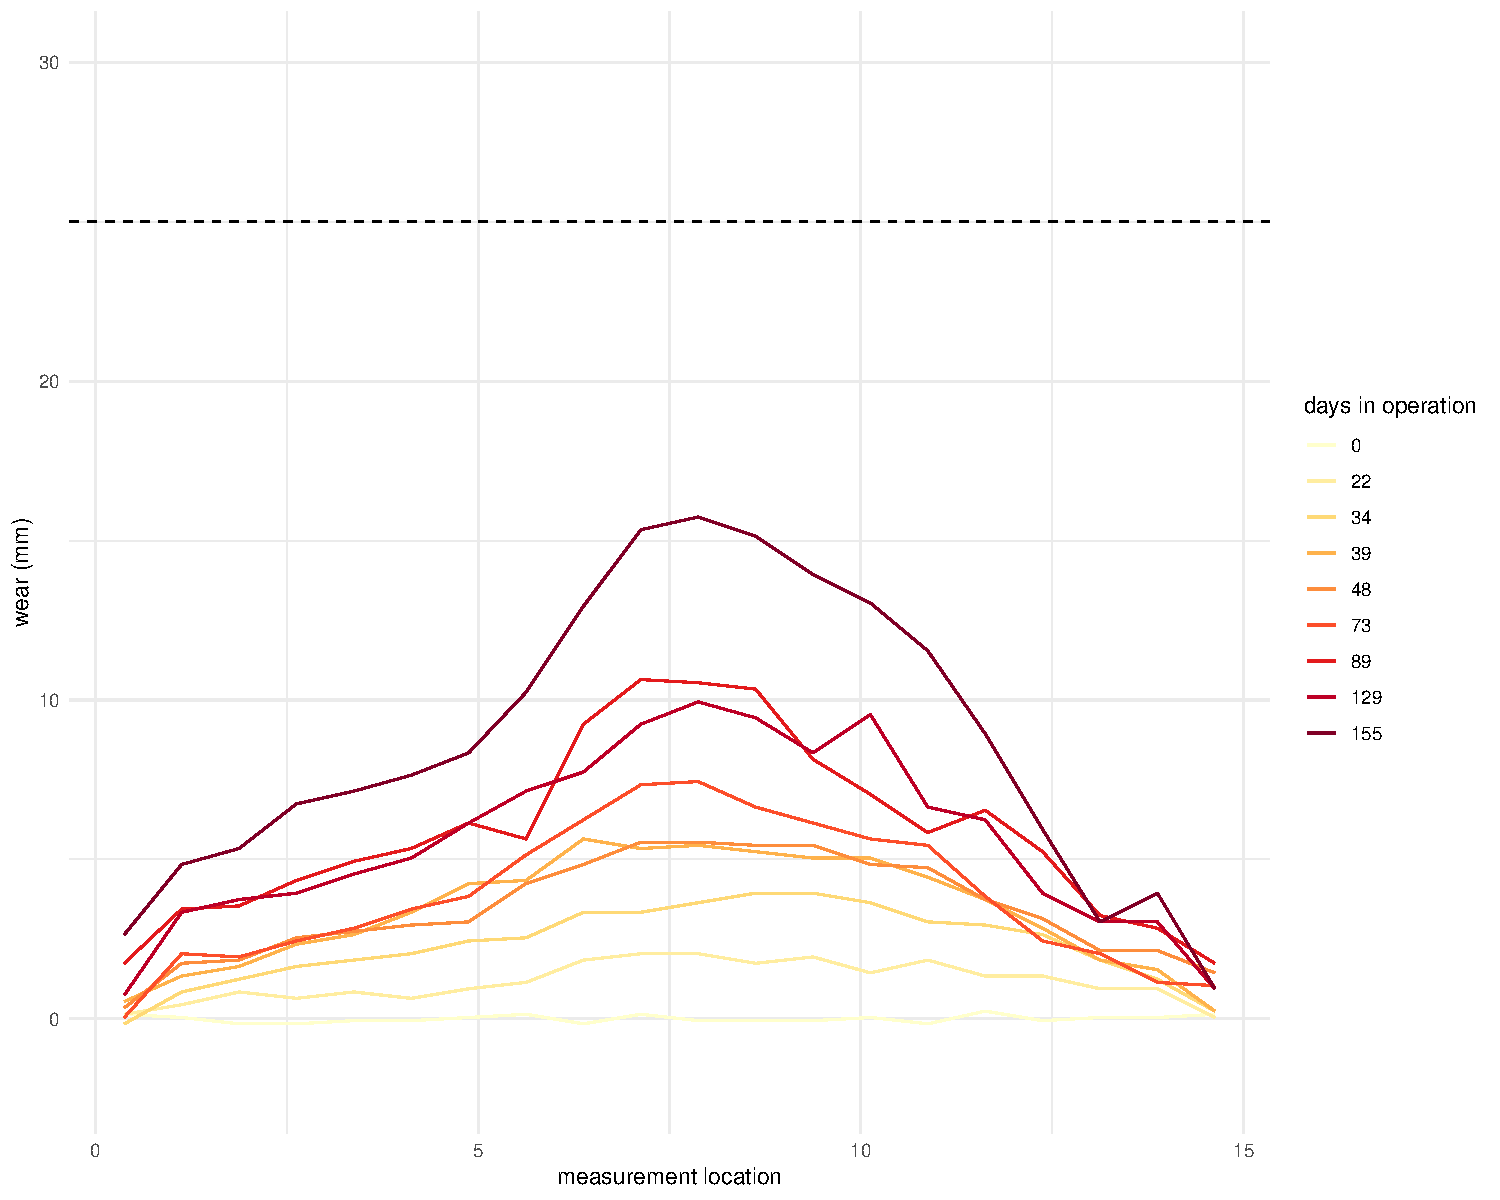
\includegraphics[width=\textwidth]{figures/ch-6/main_belt.pdf}
  \caption{The growing wear profile of a conveyor's belt over time. Ultrasonic thickness measurements are taken at $N = 20$ measurement locations across the width of the belt at repeated times. The vertical axis is wear in \textit{mm}, calculated by subtracting the measured thickness from the original thickness of the belt. The horizontal dashed line at $25mm$ of wear indicates the maximum allowable wear before the belt needs to be replaced, i.e. the soft failure threshold. The colour gradient indicates the time the belt has been in operation. Measurements taken at the beginning of the belt's life are shown in light yellow, and the most recent set of measurements are plotted in dark red}
  \label{fig:ut-example}
\end{figure}

Although there are papers that address the condition monitoring of conveyor belts, for example, identification of damage from puncture or modelling cord damage \citep{bortnowski_2022}, very few academic works focus on wear from abrasion. This is surprising considering that wear is a major failure mode of the belt \citep{bortnowski_2022}, especially for shorter, highly-utilised belts like stackers and reclaimers (which are also highly critical and difficult to maintain). \citet{webb_2020} demonstrate one typical method that an engineer would use to estimate when the failure of the belt will occur due to wear. For each measurement location along the belt's width, the engineer fits a linear relationship to the UT measurement at that location using cumulative tonnes as the predictor variable. Next, at the location with the most aggressive wear rate—--the steepest gradient—--they extrapolate the line up to some predetermined soft failure threshold, indicated by a dashed line at $25mm$ of wear in \textit{Figure}~\ref{fig:ut-example}. The time at which the extrapolated line intersects the soft failure threshold is the predicted failure time. An alternative but similar approach is to take the maximum wear measurement from each profile and fit a linear relationship to these maximum wear measurements. This second approach is used by some conveyor condition monitoring software. \textit{Figure}~\ref{fig:linear-trend-demo} demonstrates these two methods using the data in \textit{Figure}~\ref{fig:ut-example}. Unfortunately, these method neglects the many sources of uncertainty in the data-generating and observation processes. Firstly, trend fitting of the raw UT measurements is sensitive to noise in the data, especially early on in the belt's life when there are few observations. Secondly, there is no formal structure for managing the different sources of uncertainty, for example, uncertainty in the UT measurements due to measurement error, uncertainty in the wear profile because of spatial variation along the length of the belt, uncertainty in the wear rate due to variations in operating conditions, and uncertainty in the parameters of the degradation process. Finally, the prediction is based solely on the forecast from only a few measurements on that particular belt with no uncertainty quantification. Therefore, the engineer cannot quickly assess the future wear of the entire belt surface, nor can they interpret risk, which limits their ability to justify and defend their maintenance decisions.

\begin{figure}[h]
  \centering
  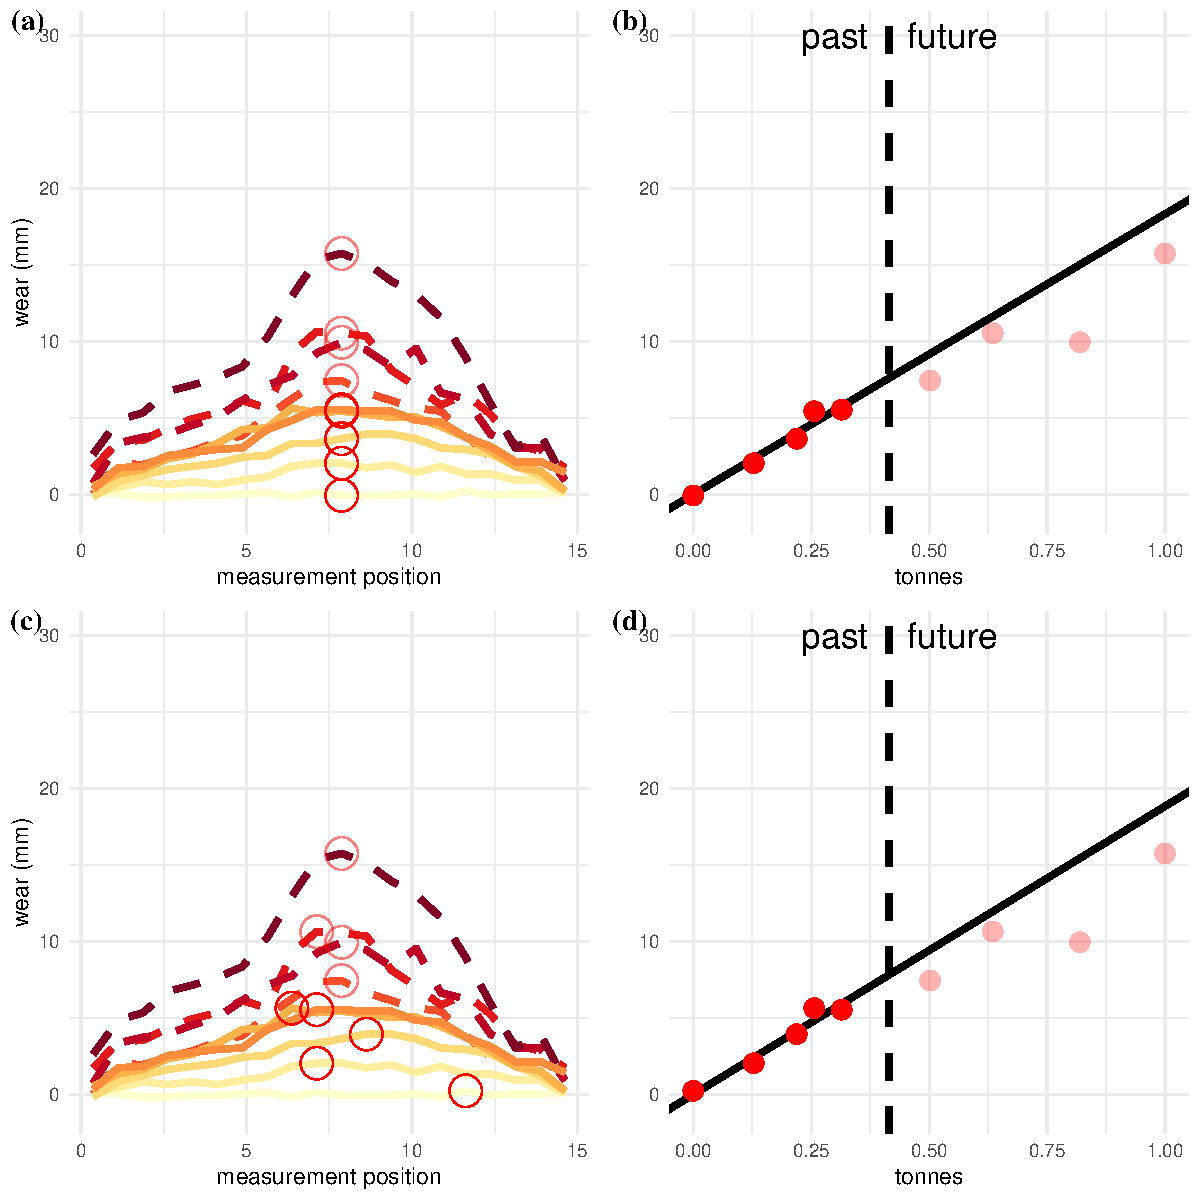
\includegraphics[width=0.7\textwidth]{figures/ch-6/current_approach.pdf}
  \caption{A demonstration of some typical approaches used to trend belt wear. (a) and (b) demonstrate the method of \citep{webb_2020}, where the measurements at the fastest wearing location which are circled in (a) are trended into the future in figure (b). (c) and (d) demonstrate an alternative but similar approach used by some reliability software, where the maximum wear measurement in each profile is trended instead.}
  \label{fig:linear-trend-demo}
\end{figure}

Rather than forecasting the wear at a single measurement location or only for the maximum wear measurement, I propose a Bayesian hierarchical method for forecasting the evolution of the entire wear profile of the belt through time. The method I use expands degradation models, such as the previous work in chapters~\ref{chap:chapter4}, and~\ref{chap:chapter5}, to functional time series. In the first level of the hierarchical model, I apply a functional data analysis (FDA) approach to modelling the condition monitoring data in Figure~\ref{fig:ut-example}. The FDA interpretation smooths the observations, which helps account for measurement error in the UT testing process; it also reduces the dimension of the data, making it easier to model the degradation at all the measurement locations simultaneously without too much of a computational burden. This functional data model, when paired with a suitable process model for the underlying degradation---either general path or stochastic process---and a suitable parameter model, formally manages the different sources of uncertainty. The proposed method produces forecasts of the belt's wear that:
\begin{enumerate}
  \item properly quantifies the uncertainties in the prediction, and
  \item produces an intuitive forecast of the entire wear profile.
\end{enumerate}
The method is not limited to conveyor belt wear; it can be used for any degrading surface monitored over a grid of locations. Here, I show an application for a one-dimensional profile, but the method could be expanded to two.

I begin in Section~\ref{sec:belt-wear-fda} by providing a brief overview of functional data analysis and showing how it can form the data model in a Bayesian hierarchical model for degradation. I then define two process models for the degradation of the belt in Section~\ref{sec:belt-wear-process}: a noisy gamma process and a linear general path. In Section~\ref{sec:belt_wear_priors}, I define the prior distributions for the two models, show how an informative prior can be constructed from historic belt wear datasets, and check the plausibility of the process model through prior predictive simulation. Section~\ref{sec:belt-wear-fitting} describes sampling and investigates the posterior draws from each model in terms of the marginal posterior distributions of the parameters, the posterior distribution of the intermediate quantities in each model that describe the underlying wear process, and the prior predictive distributions for replications of the data in Fig.~\ref{fig:ut-example}. In Section~\ref{sec:belt-wear-forecast}, I describe how to generate forecasts for the belt's wear profile using the two different models and demonstrate with the ninth wear profile observation that I withhold when fitting the two models. I then evaluate and compare the two models based on their ability to predict the degradation of the belt at future time points in Section~\ref{sec:belt-wear-comparison}. Lastly, in Section~\ref{sec:belt-wear-ft}, I demonstrate how to construct failure time distributions for the two models conditioned on the current condition of the belt. I finish in Section~\ref{sec:belt-wear-discussion} by revisiting the main results and pointing out areas of useful future work.

\section{Functional data analysis (the data model)} \label{sec:belt-wear-fda}
In functional data analysis, the data in each observation are considered as coming from a smooth underlying random function rather than being a scalar or vector-valued random variable \citep[p. 512]{BDA2020}. That is, we interpret the set of UT measurements at each observation time as noisy observations at discrete locations of some smooth underlying random function
\begin{equation}
  z_{i, n}|f_i(n),\sigma \sim N(f_i(n), \sigma).
  \label{eq:fda}
\end{equation}
In this way, the standard deviation $\sigma$ describes the noise in the UT measurement process---which we assume to be normally distributed---and the function $f_i(n)$ describes a smooth wear profile across the width of the belt at time $t_i$. The aim of a functional data analysis is, therefore, to model the collection of functions $\{f_i(.)\}^I_{i = 1}$. To do so requires the analyst to choose a functional form for $f_i(.)$, a decision on which the model is implicitly conditioned. In this analysis, I use a B-spline to model the wear profiles of the conveyor belt.

\paragraph{B-splines}
B-splines are piecewise continuous functions \citep[p. 33-38]{ramsay_2009} that are constructed as the weighted sum of a set of $M$ locally defined polynomial B-spline basis functions,
\begin{equation}
 f_i(n) = \sum_{m = 1}^{M} y_{i, m}b_m(n).
  \label{eq:spline}
\end{equation}
Here, $y_{i, m}$ is the weight of the $m^{th}$ basis function, $b_m(.)$, for the $i^{th}$ observation. The number of basis functions and their shapes and locations are defined by a set of knots and the order of the basis functions. To describe the wear profiles, I use eight evenly spaced knots and third-order basis functions. However, I also drop the outer two sets of basis functions to constrain how flexible the spline can be towards the edges of the belt and to ensure that the wear profile is fixed at zero at the boundaries. These choices were made by measuring the goodness of fit for many different conveyor wear profiles from the industry partner's condition monitoring system and weighing up simplicity and flexibility. Figure~\ref{fig:basis-functions}~(c) shows the set of un-weighted basis functions on which we condition our model. The spline is fit to the UT data by estimating the weights each basis function. As an example, Fig.~\ref{fig:basis-functions}~(a) shows the fitted spline for the fifth observation and Fig.~\ref{fig:basis-functions}~(b) shows the weighted set of basis functions that make up the wear profile. Fitting a B-spline to each set of UT measurements using the set of basis functions in Fig.~\ref{fig:basis-functions}~(c) yields the set of spline coefficients $\{y_{i, m}\}^M_{m = 1}$ that fully describes the wear profile at time $t_i$. The next level of the BHM, the process model, models how these spline coefficients evolve through time.

\begin{figure}[h]
  \centering
  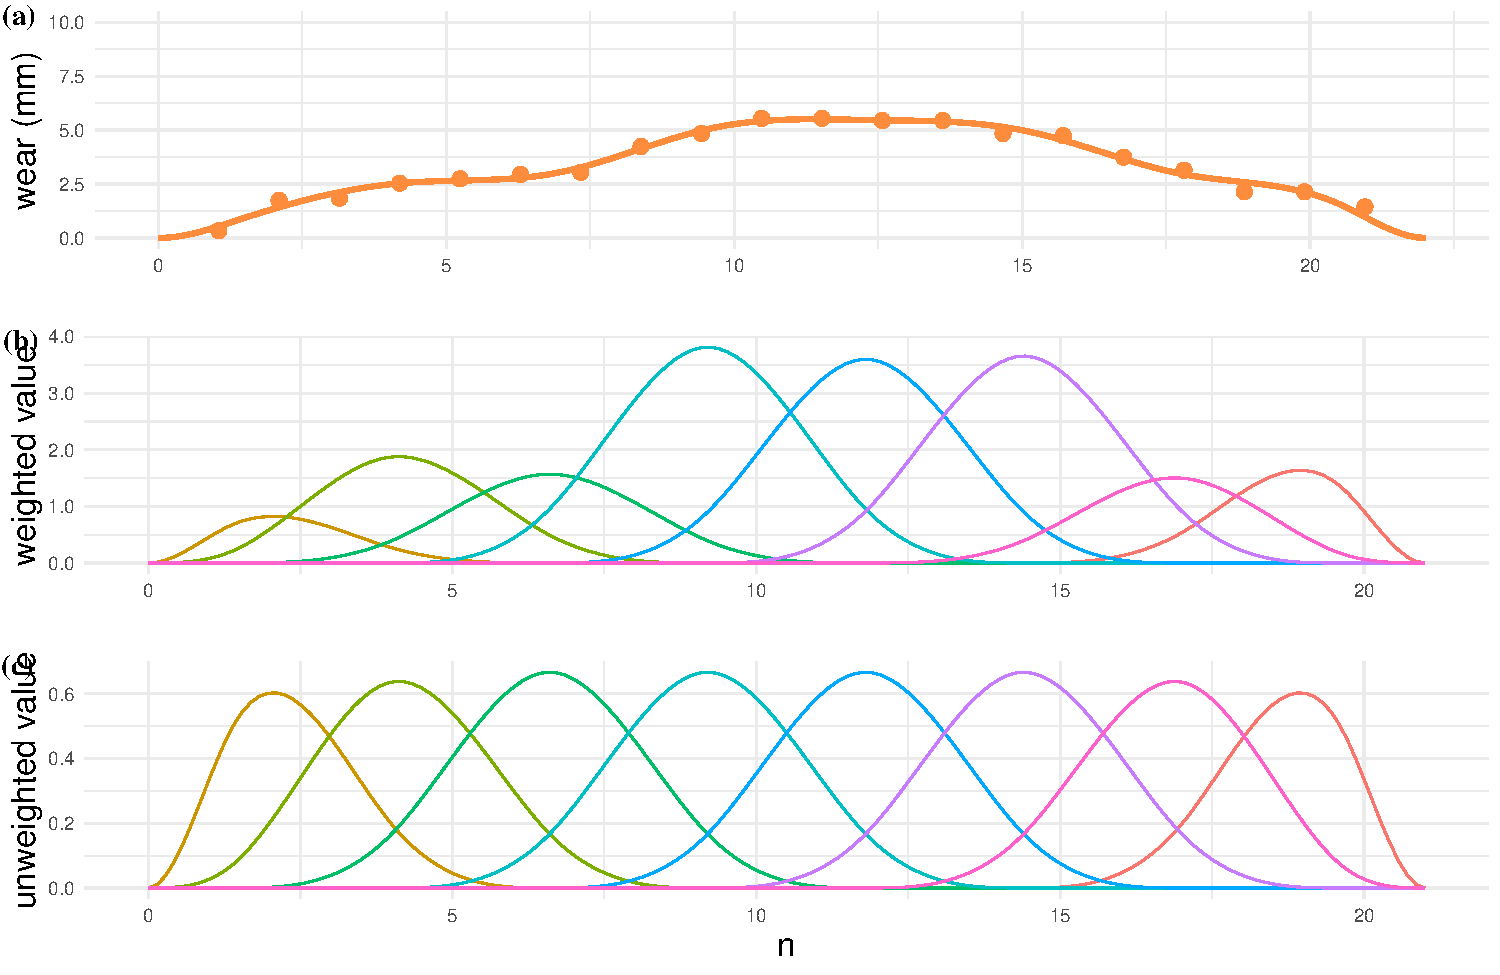
\includegraphics[width=0.9\textwidth]{figures/ch-6/b-spline-fitting.pdf}
  \caption{(a) shows a fitted wear profile for the fifth observation; (b) shows the weighted set of basis functions that make up the profile in (a); and (c) shows the unweighted set of basis functions}
  \label{fig:basis-functions}
\end{figure}

\paragraph{Functional time series}
Before moving on, I note that modelling the evolution of spline coefficients through time is not new. Functional time series analysis is an area of statistics that models how time-ordered functional observations evolve \citep{hormann_2012}. It has also been done in a Bayesian context \citep{kowal_2017}. Usually, these methods use functional PCA \citep[p. 16]{ramsay_2009} and, for the most part, autoregressive processes to model the evolution of the eigen weights (the coefficients of the eigenfunctions). Using functional PCA first reduces the number of coefficients to model. Furthermore, because the eigenfunctions are orthonormal, the eigen weights can be modelled independently. This dimension reduction is helpful for cases where many basis functions are needed to fit the data because, in these cases, modelling the basis coefficients directly would require a very large covariance matrix. However, in our case, the number of functional observations of the belt is too small to perform PCA reliably, and the degradation process is not stationary. Rather, we use a degradation model to model the spline coefficients directly and, for the moment, assume that the coefficients are independent of one another. In this way, our approach may be more down the path of the spatio-temporal models of \citet[p. 218-224]{wikle_2019}.

\section{Process models} \label{sec:belt-wear-process}
As potential process models for the underlying degradation process of the belt, I explore both a noisy gamma process and a linear general path model. In the noisy gamma process model, I model the spline coefficients with effectively the same model that I presented in chapters~\ref{chap:chapter4}, and~\ref{chap:chapter5}, except with some minor adjustments to make the model more robust to outlying observations. In the linear path model, I use a much simpler linear model for the spline coefficients. The major difference between the two process models is that the noisy stochastic process model explicitly breaks down the variation in the degradation signal into variation attributed to changes in degradation rate through time---which could arise from changes in operation or environmental conditions---and the uncertainty of the measurement process---which in this case arises because the cross-section is not always measured in the same location. In contrast, the general path model assumes that the degradation path is deterministic conditional on the model's parameters and the time $t$ and lumps the variability from both the variation in signal through time and measurement error into a single error term. When using a general path model, additional structure in the noisy degradation measurements can be accounted for by adjusting the error distribution, for example, adding autoregressive error terms. In some cases, the two approaches are directly comparable; for example, \citet{whitmore_1995} formulates a Weiner degradation process with measurement error as a multiple linear regression with added covariance structure. Some discussions of stochastic process and general path models can be found in \citet{ye2015}. The benefit of using the noisy gamma process, in this case, is that by modelling these two sources of variation separately, we can assign them different distributions (Gaussian-distributed measurement error and gamma-distributed jumps), which explicitly splits up the two sources of uncertainty. However, there may be a limit of measurement error and/or volatility of the degradation process where it is simpler and better to use the general path model even though it is less physically motivated. Below, I outline the two process models.

\subsection{Noisy gamma process}
In the gamma process version of the process model, I model each spline coefficient as coming from a $\mbox{t}$ distribution with $10$ degrees of freedom where the location depends on the estimated `average' value of the spline coefficient along the length of the belt at that time and the scale depends on the estimated average value and scale parameter $\phi$. Assuming a $\mbox{t}$ distribution for the spline coefficients makes the model more robust to outlying observations \citep[Chapter~17]{BDA2020}. I then model the progression of the `average' degradation of the spline coefficient through the gamma process parametrised in terms of the mean and coefficient of variation
\begin{align*}
  y_{m, i}|y^*_{m, i}, \phi      \sim & \mbox{t}_{10}\left(y^*_{m, i}, \phi y^*_{m, i}\right)                       \\
  \Delta  y^*_{m, i}                = & y^*_{m, i} - y^*_{m, i-1}                                                   \\
  \Delta y^*_{m, i}|\nu_m, \mu_m \sim & \mbox{Ga}\left( \frac{\Delta t_i}{\nu_m^2}, \frac{1}{\mu_m \nu_m^2} \right).
\end{align*}
In this process model, each of the $m$ spline coefficients has specific $\mu_m$ and $\nu_m$.

\subsection{Linear model}
In the linear general path version of the process model, I use the same $\mbox{t}_{10}$ structure to model the noisy spline coefficients conditional on their estimated average value and $\phi$, but now model the progression of the average value of each spline coefficient as a deterministic function of $t$ that is specified in terms of the average wear rate $\mu_m$
\begin{align*}
  y_{m, i}|y^*_{m, i}, \phi \sim & \mbox{t}_{10}\left(y^*_{m, i}, \phi y^*_{m, i}\right)  \\
  y^*_{m, i}                   = & \mu_m t_{i}.
\end{align*}

\section{Parameter model} \label{sec:belt_wear_priors}
Because I have used the mean/coefficient of variation parameterisation of the gamma process and a conditional structure for both the models, they share many of the same parameters---$\sigma$, $\phi$, and the $\mu_m$. Hence, I use the same priors in both models. For the variance parameters $\sigma$ and $\phi$ I use the priors
\begin{align*}
  \sigma \sim & \mbox{U}(0, 100)         \\
  \phi   \sim & \mbox{Cauchy}^{+}(0, 25)
\end{align*}
based on the same justifications presented in Section~\ref{sec:GP_priors} \citep[chap.~17]{BDA2020}. For the mean wear rate of the different spline coefficients, I now use the prior 
\begin{equation*}
  \mu_m \sim \mbox{N}(\hat{a}, \hat{b})
\end{equation*}
where $\hat{a}$ and $\hat{b}$ are estimated from historic data. I go into more detail on how this is done below, but first, define the remaining priors for the gamma process.

The gamma process model has slightly more parameters than the simpler linear path model. For the coefficient of variation parameters $\nu_m$, I use the hierarchical prior
\begin{align*}
  \nu_m      \sim & \mbox{N}(\mu_\nu, \sigma_\nu) \\
  \mu_\nu    \sim & \mbox{t}_3(0, 0.5)            \\
  \sigma_\nu \sim & \mbox{Cauchy}^{+}(0, 0.25)
\end{align*}
defined in the same way as the unit-to-unit variability model in Section~\ref{subsec:partial-pooling}. The hierarchical prior partially pools information between the $\nu_m$ of the gamma processes for each spline coefficient (because they all belong to the same belt we expect them to be similar) while still allowing them to vary.

\paragraph*{Choosing informative hyperparameters for $\mu$} There are also historic belt wear datasets for the particular conveyor that the data in Fig.~\ref{fig:ut-example} come from. Two of these historical datasets are shown in Figure~\ref{fig:previouse-belts}. According to the industry partner from whom we got the data, the future wear behaviour of the belt is expected to be different from the historic wear datasets because of variations in ore composition, belt manufacturer, and operational strategies. However, the historic wear behaviour of the belt should indicate future behaviour. Although the historical data cannot be directly used in the analysis, in the Bayesian framework, the historical data can be used to formulate an informative prior and, therefore, still supplement the analysis.

\begin{figure}
  \centering
  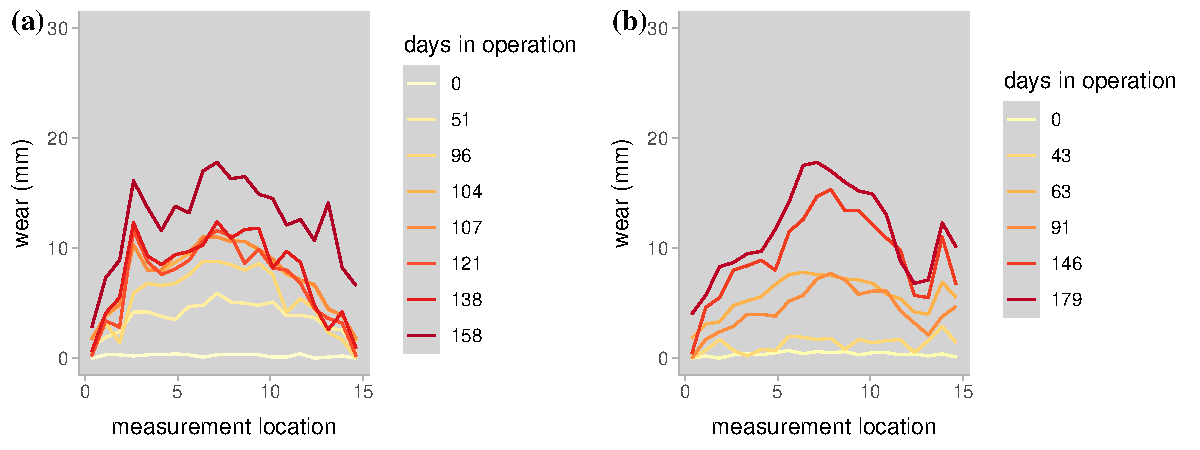
\includegraphics[width=\textwidth]{figures/ch-6/historic_belts.pdf}
  \caption{Two historic belt wear data sets from the same conveyor}
  \label{fig:previouse-belts}
\end{figure}

I encode the prior information in the model through the parameter $\mu$. To do so, I fit B-splines to each of the historic wear profiles using the same set of basis functions in Fig.~\ref{fig:basis-functions}~(c) to calculate the spline coefficients and then estimate the average wear of each coefficient. Figure~\ref{fig:inf-prior-mu} shows the linear regressions for each spline coefficient. Based on the estimates, I set $\hat{a}_m$ in the prior for $\mu_m$ as the estimated slope of the coefficient based on the historical data and $\hat{b}_m$ as five times the standard error of the estimate.

\begin{figure}
  \centering
  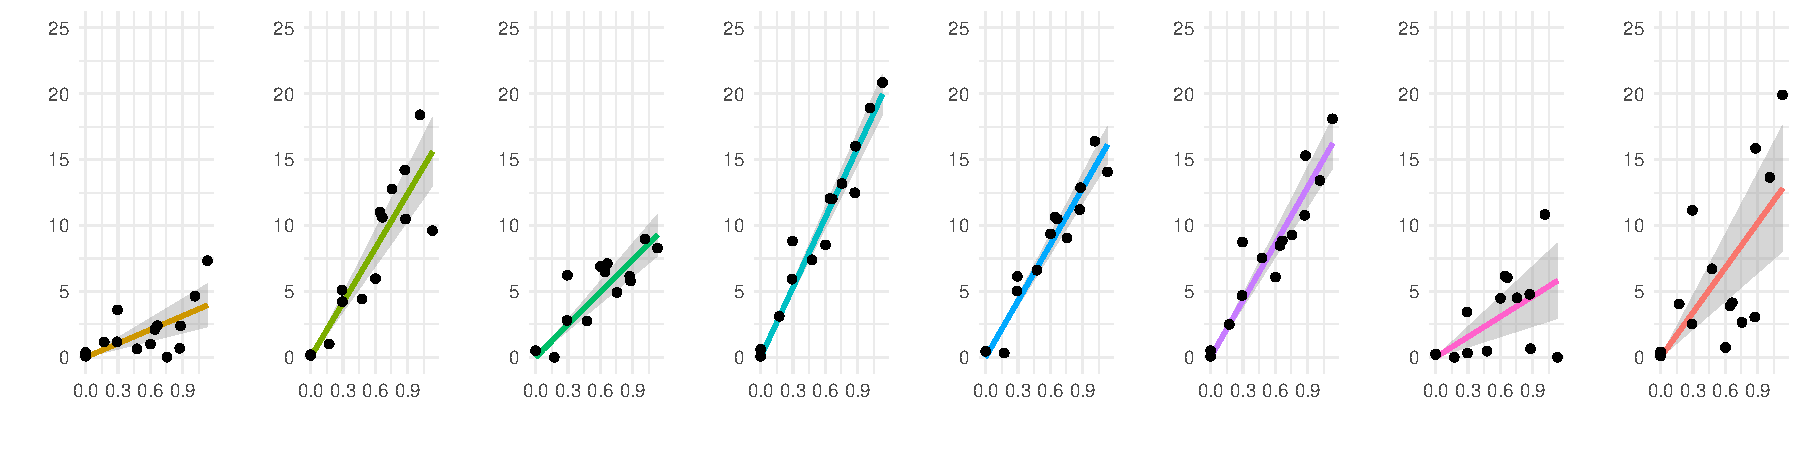
\includegraphics[width=\textwidth]{figures/ch-6/informative-prior-mu.pdf}
  \caption{The estimated average wear rate for each spline coefficients calculated from the datasets in Fig.~\ref{fig:previouse-belts}. The colour of each fit corresponds to the basis functions in Fig.~\ref{fig:basis-functions}~(c). The horizontal scale of each plots is in tonnes and the vertical scale is the value of the spline coefficient.}
  \label{fig:inf-prior-mu}
\end{figure}

\paragraph*{Prior predictive checking} 

To check the plausibility of the proposed priors in the context of the two process models, I perform prior predictive checking. Figure~\ref{fig:prior-pc-beltwear} shows sixteen prior predictive simulations from the gamma process (solid lines) and linear model (dashed lines). Because I have used very vague priors for the parameters $\sigma$ and $\phi$, simulating the noisy wear profiles and UT measurements will not make sense until after conditioning on the observed data. Therefore, the simulations shown in Fig.~\ref{fig:prior-pc-beltwear} are for the belt's non-noisy (average) wear profile.

\begin{figure}
  \centering
  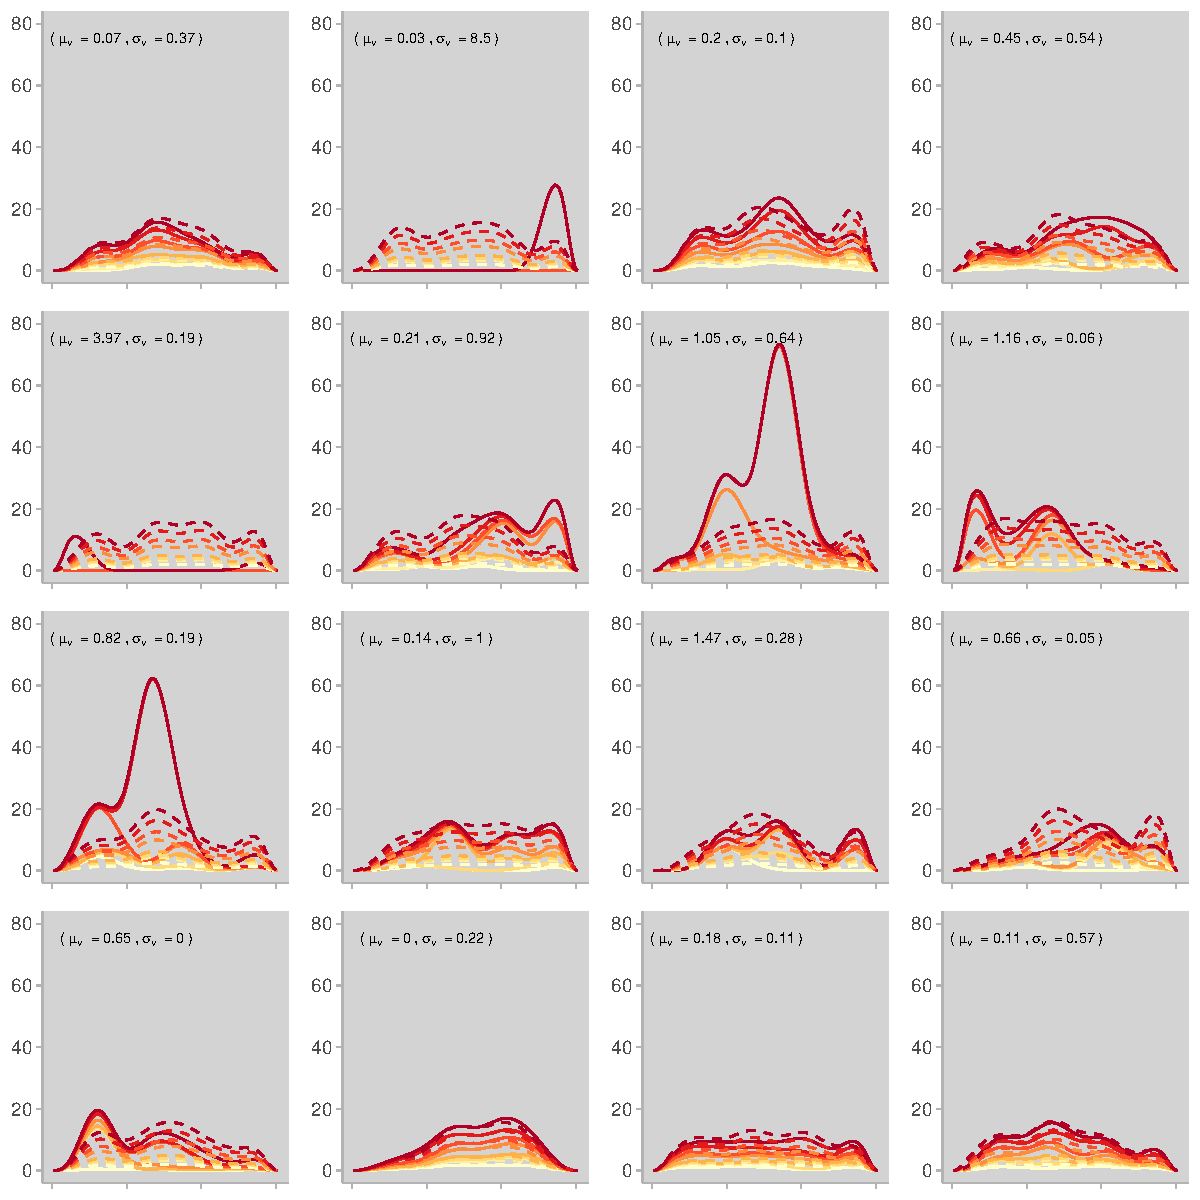
\includegraphics[width=\textwidth]{figures/ch-6/prior-pc.pdf}
  \caption{Sixteen prior predictive simulations of the average wear profile generated from the linear path (dashed line) and gamma process (solid line) process models with the priors defined in Sec.~\ref{sec:belt_wear_priors}. The values of the hyper parameters for $\nu$ in the gamma process that were used to generate each simulation are displayed on each plot.}
  \label{fig:prior-pc-beltwear}
\end{figure}

To generate each fictitious data set, I sample a value of each $\mu_m$, $\mu_\nu$, and $\sigma_\nu$ from their prior. I then sample the values of $\nu_m$ from the hierarchical prior using the realisation of $\mu_\nu$ and $\sigma_\nu$. Next, I generate values of the smoothed spline coefficients for each observation time $t_i$ from each of the two process models and apply the coefficients to the set of basis functions to calculate the smooth wear profiles. For the linear general path model, this means simply multiplying each of the $\mu_m$ by each $t_i$ to get the values of the spline coefficients. Whereas, for the gamma process, I simulate the sets of jumps in degradation using the distributions $\mbox{Ga}(\Delta t_i/\nu_m^2, 1 / (\mu_m \nu_m^2))$ and take the cumulative sum to calculate the values of the filtered spline coefficients.

The fictitious data resulting from each model, for the most part, look somewhat realistic in scale and shape. Some of the gamma process simulations look unrealistic---there are some where the wear jumps $60mm$ between observation times and others where the belt does not wear at all---but many look sensible. The shapes of most of the linear simulations look reasonable, but their growth looks synthetic and not natural enough---this should change when I add in the noise layer. In each plot, I have used the same set of realisations of the $\mu_m$ to simulate from both the gamma process and linear general path model. The realised values of the hyperparameters of the hierarchical prior for the $\nu_m$ used in the gamma process models are displayed in each subplot. Notice that when $\mu_\nu \text{ and } \sigma_\nu \longrightarrow 0$ the profiles from the gamma process match those from the linear model very closely and when the values of the hyperparameters allow for large values of the $\nu_m$---i.e. when either $\mu_\nu$, $\sigma_\nu$, or both are large---the simulated data from the gamma process model look unrealistic. However, in these simulations, the gamma process model looks to be able to generate the most natural-looking datasets. One thing of note is that many of the simulations, particularly for the gamma process, appear unrealistically wiggly. This `wiggliness' is due to a lack of large-scale spatial structure in the model and is a feature of the postulated model, not the prior. Incorporating large-scale spatial structure could be addressed in future works, but I do not address it here since this behaviour is `smoothed out' when all the possible curves are interpreted as a distribution. All in all, the simulations from both models are in the realms of plausibility, which is what is desired of a weekly informative prior \citep{gabry_vis_2019}.

\section{Posterior sampling and inference} \label{sec:belt-wear-fitting}

Conditioning on the first eight observations, I generate samples from the posterior distributions of each model using the No-U-Turn sampler implemented in \textit{Stan} \citep{Stan2022}. In total, I generated $12000$ samples from each posterior, using four chains that are $4000$ iterations in length with no thinning and a burn-in of $1000$ iterations. For the case of the gamma process, sampling results in a small number of divergent transitions---roughly $0.9\%$---which appear to arise in the hierarchical prior for the same reasons as previously discussed in Section~\ref{sec:unit-to-unit-sampling}; however, because of the very limited number of divergent transitions, I do not try and rectify the issue. The linear general path model, on the other hand, fits very efficiently without any divergent transitions, and both models show good $\hat{R}$ statistics and effective sample sizes for the parameters. In this section, I visually analyse and compare the posterior samples from each model through the marginal posterior distributions of the parameters, the posterior distributions of the intermediate quantities in the models, and the posterior predictive distributions of the UT measurements and underlying wear profiles.

\paragraph{Marginal posteriors of parameters} 
The marginal posteriors of the parameters show our updated belief after conditioning on the data. Essentially, compared with the prior, they show what we have learnt from the data. Additionally, the posterior draws of the parameters are important because we rely on them when forecasting the underlying process into the future in Section~\ref{sec:belt-wear-forecast}. Figure~\ref{fig:marginal-dist-gp-beltwear} and~\ref{fig:marginal-dist-lm-beltwear} show the marginal posterior distributions of the parameters in the gamma process and linear general path model, respectively.

\begin{figure}
  \centering
  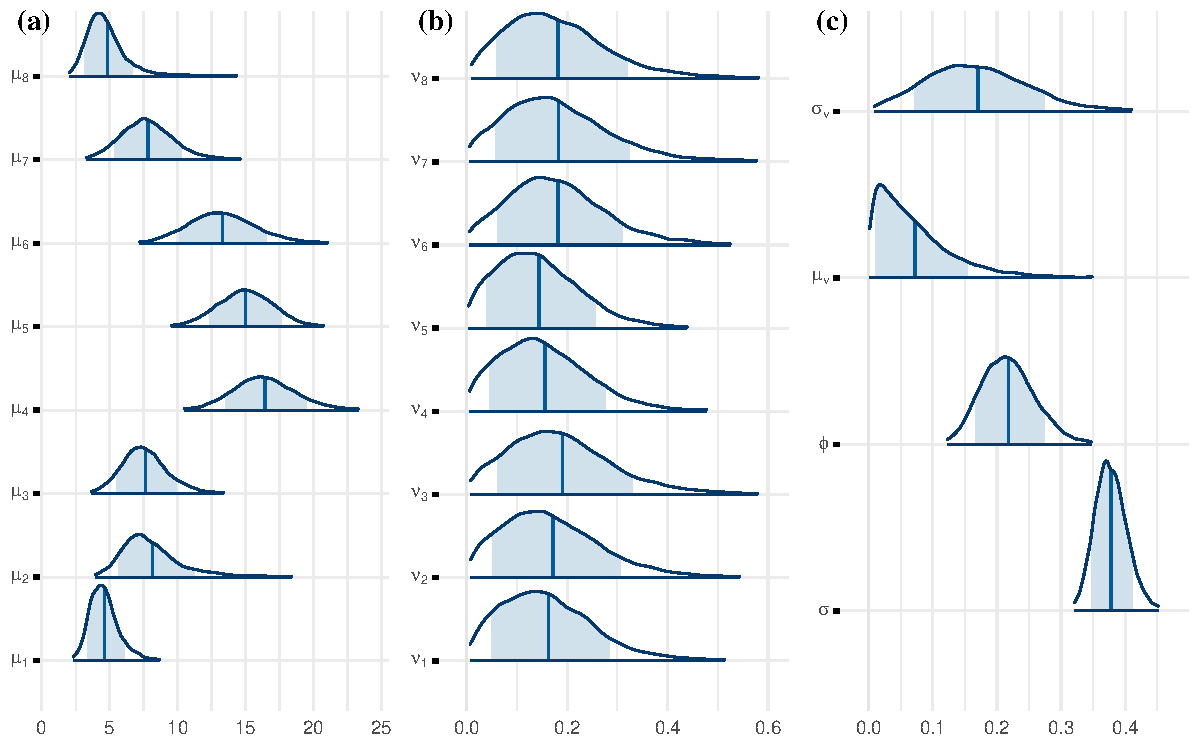
\includegraphics[width=0.8\textwidth]{figures/ch-6/marginal_post_gp.pdf}
  \caption{Marginal posterior distributions of the gamma process model parameters.}
  \label{fig:marginal-dist-gp-beltwear}
\end{figure}

In the marginal distributions of the parameters of the Gamma process model, shown in Fig.~\ref{fig:marginal-dist-gp-beltwear}, we can see three main things. Firstly, by looking at the distribution of the different $\mu_m$, Fig.~\ref{fig:marginal-dist-gp-beltwear}~(a), we can see that the model has successfully captured the belt's general `dishing out' behaviour since the mean wear rates of the spline coefficients closer to the centre of the belt are higher. Secondly, the general wear of the belt appears to be lop-sided since there is a lack of symmetry in the $\mu_m$---the posterior median of $\mu_6$ is much greater than that of $\mu_3$. These first two points may be obvious to the reader when looking at the raw data in Fig.~\ref{fig:ut-example}, but it is important that the model has identified the general behaviour as chronic and not just noise, especially when our main goal is to forecast the wear profile through time. The third main observation is how little variability there is amongst the $\nu_m$ in Fig.~\ref{fig:marginal-dist-gp-beltwear}~(b). Their expected values are very similar, and the marginal posterior of $\sigma_\nu$, shown in Fig.~\ref{fig:marginal-dist-gp-beltwear}~(c), has a lot of mass near zero. However, it is hard to say whether or not the variability is negligible.

In addition to these three main points, in Fig.~\ref{fig:marginal-dist-gp-beltwear}~(c), it looks as though the marginal posteriors of the two variance parameters $\sigma$ and $\phi$ and the two hyperparameters of $\nu$ encode similar levels of uncertainty into the model. However, this is not the case, even though the marginal posteriors have similar scales. $\sigma$ can be interpreted directly in $mm$, but the effect of $\phi$ is scaled by the values of the filtered spline coefficient and should rather be interpreted as a proportion of $y^*$. The influence of the posterior distributions of $\sigma$ and $\phi$ is much more obvious in the posterior predictive distributions. On the other hand, the uncertainty in the degradation path that results from the underlying gamma process and the posterior distribution of its parameters and hyperparameters---$\mu_\nu$, $\sigma_\nu$, $\nu_m$, and $\mu_m$---is almost impossible to interpret from the marginal distributions in Fig.~\ref{fig:marginal-dist-gp-beltwear}. We gain a better intuition of the uncertainty in the underlying gamma degradation process by looking at the marginal posterior of the filtered spline coefficients $y^*_{i, m}$. I look at the posterior distributions of these intermediate quantities and the posterior predictive distributions next, but first, I compare the marginal posteriors from the fitted general path model to the marginal distributions from the gamma process that I have looked at here.

\begin{figure}
  \centering
  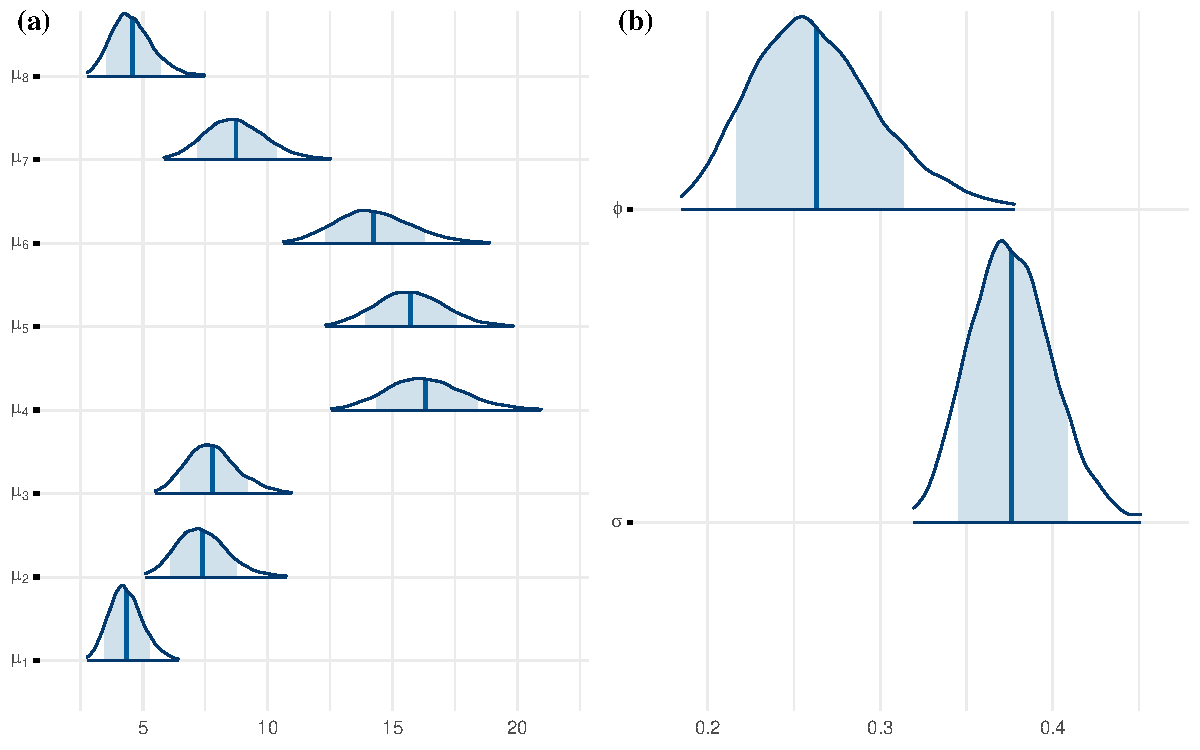
\includegraphics[width=0.8\textwidth]{figures/ch-6/marginal_post_lm.pdf}
  \caption{Marginal posterior distributions of the linear general path model parameters.}
  \label{fig:marginal-dist-lm-beltwear}
\end{figure}

Figure~\ref{fig:marginal-dist-lm-beltwear} shows the marginal posteriors of parameters in the general path model. The marginal posterior distributions of the $\mu_m$ from the general path model in Fig.~\ref{fig:marginal-dist-lm-beltwear}~(a) show the same general dishing out behaviour of the belt and asymmetric wear pattern. In fact, comparing Fig.~\ref{fig:marginal-dist-lm-beltwear}~(a) with Fig.~\ref{fig:marginal-dist-gp-beltwear}~(a), it appears that the posterior distribution of the $\mu_m$ are almost identical in the two models. The only observable difference is that the marginal distributions have heavier upper tails in the posterior of the gamma process model. In the marginal posteriors of the parameters $\sigma$ and $\phi$ in Fig.~\ref{fig:marginal-dist-lm-beltwear}~(b), the estimated value of sigma and corresponding uncertainty is also very similar to the gamma process model; however, the estimated value of $\phi$ is clearly higher. As expected, the scale of the $\mbox{t}_{10}$ distribution in the parameter model has inflated in the case of the general path model to account for the variability in the degradation rate that would otherwise be accounted for by the jumpy gamma process. The distinction between the two process models is clearest in the posteriors of the intermediate quantities in the two models.

\paragraph{Intermediate quantities}
The $y^*_{i, m}$ are the filtered degradation paths of each spline coefficient, which essentially describe the `average' wear along the length of the belt at each time. The intermediate quantities in the model are treated similarly to parameters in the Bayesian framework; as such, we also obtain posterior draws of the $y^*_{i, m}$ during MCMC sampling. Figure~\ref{fig:y-post-beltwear} shows the mean posterior value of the filtered degradation of each coefficient---plotted as coloured lines. Fig.~\ref{fig:y-post-beltwear}~(a) shows the posterior of the gamma process model, and Fig.~\ref{fig:y-post-beltwear}~(b) shows the posterior of the general path model. The colours of the mean path correspond to the basis functions in Fig.~\ref{fig:basis-functions}~(c). One hundred individual draws from each of the joint posteriors of the $y^*$ are also plotted in Fig.~\ref{fig:y-post-beltwear} as dark grey lines.

The draws of the spline coefficient from the gamma process mode in Fig.~\ref{fig:y-post-beltwear}~(a) are noticeably `jumpy' while the mean paths of the filtered spline coefficients look reasonably linear. For the general path model in Fig.~\ref{fig:y-post-beltwear}~(b), on the other hand, all of the posterior draws are perfectly straight lines. Despite this difference, the spread of the draws of the pathways in each equivalent subplot in Fig.~\ref{fig:y-post-beltwear}~(a) and~(b) are very similar. The fact that most of the draws from the gamma process appear as jumpy processes---even though we specified a prior which favours straight processes--- seems to suggest that the wear rate varies through time, and as such, we should allow the model to do so too. The general path model has accounted for this added variability in the data by inflating the value of $\phi$, as we previously noted. This difference is why some argue that the gamma process is a more realistic and physically motivated model \citep{ye2015}. However, the simplification of reality that linear models apply is notoriously successful. To understand if the simplified linear model is flexible enough to sufficiently describe the data and if the data contain enough information and a clear enough signal to identify the gamma process with its extra parameters, I look at the posterior predictive distributions for the two different models and compare them with the observed data.

\begin{figure}
  \centering
  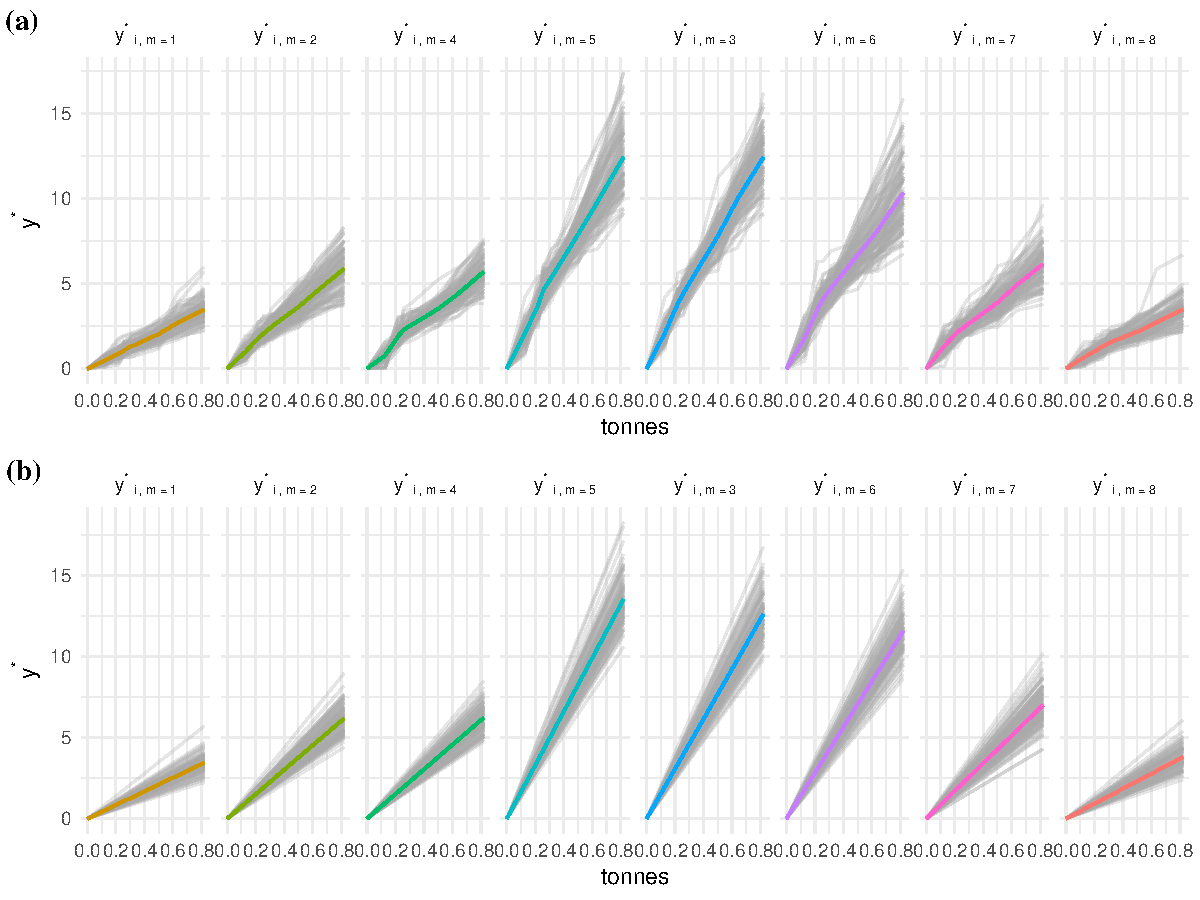
\includegraphics[width=0.9\textwidth]{figures/ch-6/post_y_belt_wear.pdf}
  \caption{The posterior draws of the filtered spline coefficients for (a) the gamma process model and (b) the linear general path model.}
  \label{fig:y-post-beltwear}
\end{figure}

\paragraph{Posterior predictive distributions}

As discussed in section~\ref{sec:bayesian-background}, a method for checking the fit of Bayesian models is to check if the data look plausible under posterior predictive distribution. In hierarchical models, this comparison can be performed at different levels of the model to check the fit of the data model and process models. Here, I generate a compare the posterior predictive distributions of replications of the UT measurements at the same times and locations along the belt as the data in Fig.~\ref{fig:ut-example} as well as the predictive distribution of replications of the wear profile at different locations along the belt's length at the same observation times.

To generate posterior predictive distributions for replications of the UT measurements, $\tilde{z}$, I sample from the data model conditional on the draws of the spline coefficients and $\sigma$
\begin{equation}
  \tilde{z}_{i, n}|\underline{y}_{i}^s, \sigma^s \sim \mbox{N}\left(f^s_i(n), \sigma^s\right).
\end{equation}
The posterior predictive distribution is generated in the same way for both models. The joint posterior predictive distribution of $\tilde{z}$ from the gamma process model is shown in Fig.~\ref{fig:post-pred-dists-beltwear}~(a), and from the general path model in Fig.~\ref{fig:post-pred-dists-beltwear}~(c). The observed data are also plotted in both sub-plots for comparison. At the noisy UT observation levels, the prior predictive distributions of $\tilde{z}$ for both models are very similar and fit the observed data well. In both cases, all of the observed UT data sit very close to the median wear profiles (showing that the models are flexible enough to fit the data) and sit neatly within the $95\%$ uncertainty intervals. 

To generate the posterior predictive distribution for replications of the measured wear profiles at each observation time, I sample new values of the noisy spline coefficients from the first level of the process model conditioned on the posterior draws of the filtered (mean) values of the spline coefficients and $\phi$,
\begin{equation}
  \tilde{y}_{i, m}|y^{*s}_{i, m}, \phi^s \sim \mbox{t}_{10} (y^{*s}_{i, m}, \phi^s y^{*s}_{i, m}),
\end{equation}
and then calculate the values of the spline functions $f_i(n) = \sum^{M}_{m = 1}b_m(n)\tilde{y}_{i, m}$. This process is also the same for both models. The posterior predictive distribution of the wear profiles at each observation time generated from the posterior of the gamma process is shown in Fig.~\ref{fig:post-pred-dists-beltwear}~(b); Fig.~\ref{fig:post-pred-dists-beltwear}~(d) shows their posterior predictive distribution generated from the general path model. In Fig.~\ref{fig:post-pred-dists-beltwear}~(b) and~(d), I plot each observation time separately so that the $95\%$ uncertainty intervals are clear. In all sub-plots, the observed data are included for comparison.

In the case of the posterior predictive distribution of $\tilde{y}$, the average wear profiles of the belt at each time are now clearly monotonic increasing and the uncertainty around the average wear profile also grows with time. In both figures~\ref{fig:post-pred-dists-beltwear}~(b) and~(d), the observed noisy UT wear profiles sit inside the uncertainty intervals, showing that the observed data are also plausible under both Bayesian hierarchical models at the process model level, but comparing Fig.~\ref{fig:post-pred-dists-beltwear}~(b) and~(d), the linear model appears to predict a greater wear rate and larger uncertainty than the gamma process model.

\begin{figure}
  \centering
  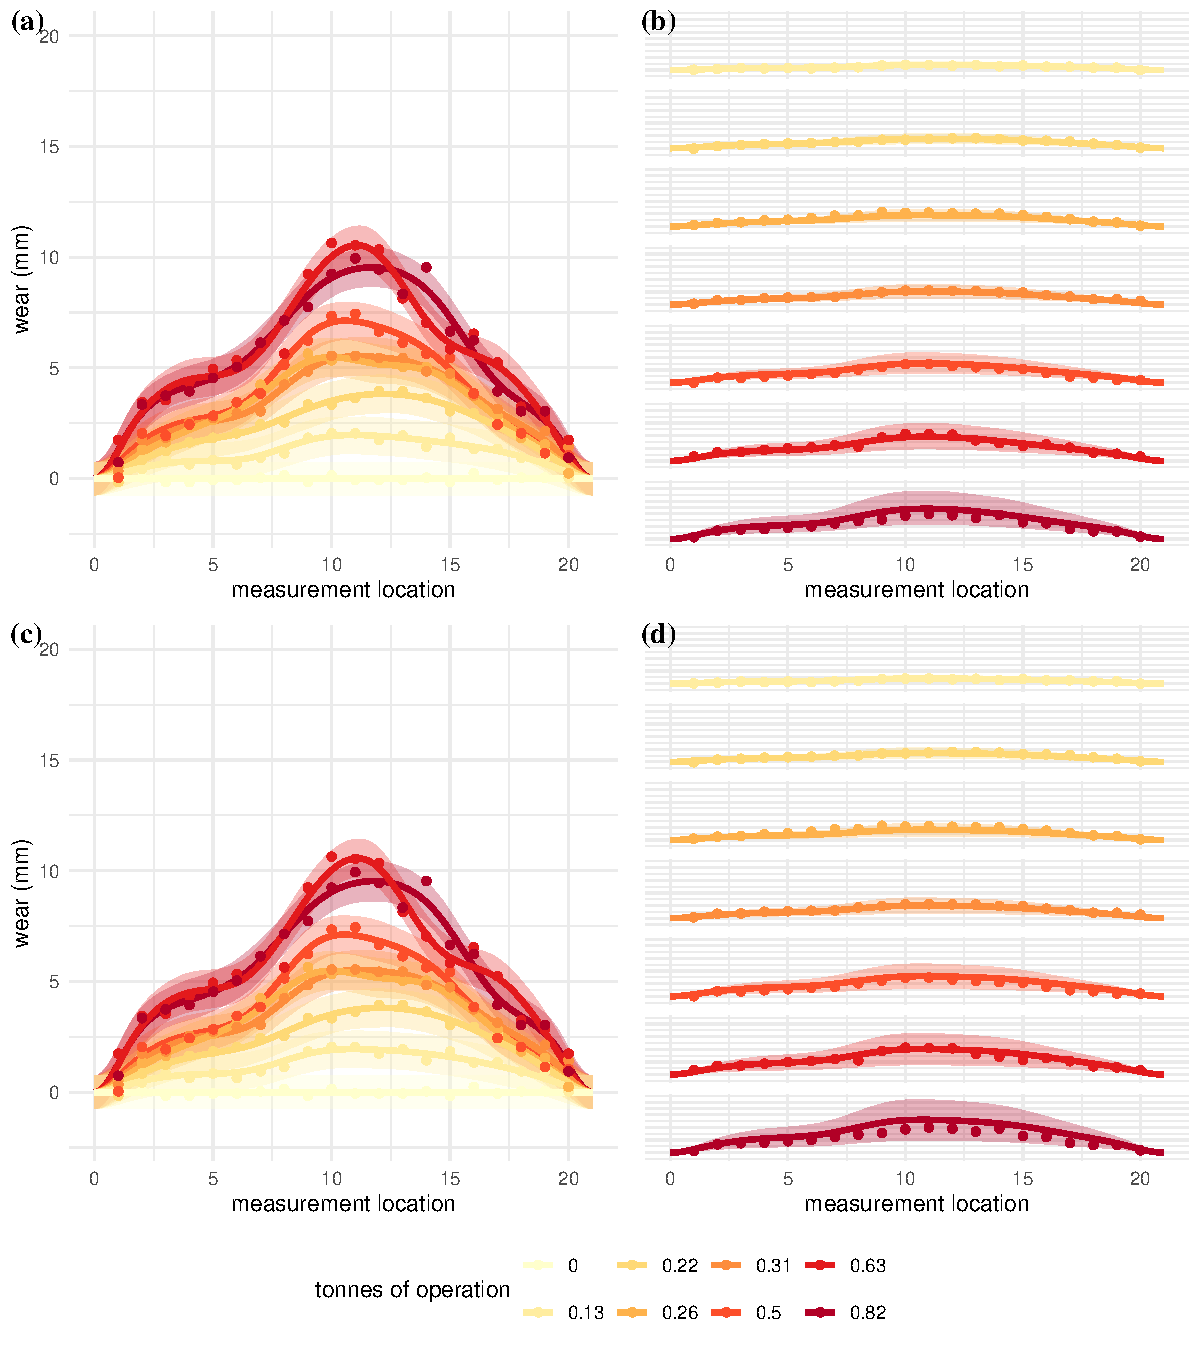
\includegraphics[width=\textwidth]{figures/ch-6/post_pred_belt_wear.pdf}
  \caption{Four posterior predictive distributions, two form each model. (a) and (c) shows the predicted smooth functional observation of the wear profiles underlying the sets of UT measurements from the gamma process and general path model, respectively. The UT measurements are also plotted as points as a reference. (b) and (d) shows the posterior predictive distribution of a new observation of the wear profile along the length of the belt at each observation time for the gamma process and general path model, respectively. In (b) and (d), the observed wear profiles are also plotted for comparison.}
  \label{fig:post-pred-dists-beltwear}
\end{figure}

\section{Forecasting degradation curves} \label{sec:belt-wear-forecast}

Using the posterior draws from the two posteriors, we can forecast the degradation process of the spline coefficients using the process model and predict the belt's wear profile at any time, $t_{I+1}$, in the future, conditioned on the belts current state of degradation. When producing the forecast, we should do so along the entire belt's length since we want to predict when any part of the belt will exceed the soft failure threshold. In other words, we want to predict the distribution of the noisy spline coefficients at the forecast time $t_{I + 1}$. The forecasts to the time $t_9 = 1$ of the ninth (withheld) belt wear observation are shown in Fig.~\ref{fig:beltwear-forecasts} for the gamma process model (a) and general path model (b) (approximately $0.18$ \textit{tonnes} or $3.7$ weeks into the future). In each sub-plot, the median forecast is shown as a solid black curve, and the $0.50$, $0.80$, and $0.95$ uncertainty intervals are shown in various shades of blue. The observed UT measurements at $t_9$---withheld from the model---are also plotted in each figure for comparison.

\begin{figure}
  \centering
  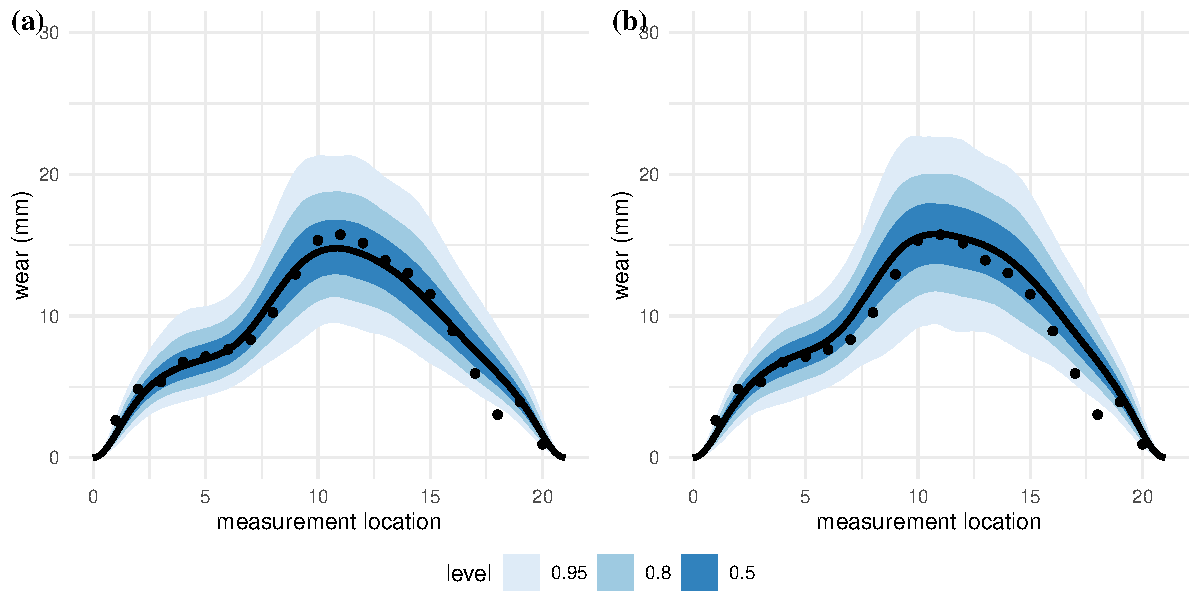
\includegraphics[width=\textwidth]{figures/ch-6/belt_wear_forecasts.pdf}
  \caption{Forecasts of the ninth, withheld, observation from (a) the gamma process model and (b) the linear general path model. The true, observed, measurements are plotted for reference.}
  \label{fig:beltwear-forecasts}
\end{figure}

The process of generating the two forecasts in Fig.~\ref{fig:beltwear-forecasts} are quite different. For the gamma process model, I first sample jumps of the spline coefficients from the gamma distribution
\begin{equation}
  \Delta y^*_{I + 1, m}|\nu_m, \nu_m, z \sim Ga\left(\frac{t_{I + 1} - t_{I}}{\nu_m^2}, \frac{1}{\mu_m, \nu_m^2}\right)
\end{equation}
using the posterior draws of the gamma process parameters. I then add these jumps to the filtered values of the spline coefficients at time $t_I$, $\{y^*_{I, m}\}^M_{m = 1}$, to predict the values of the filtered spline coefficients at time $t_{I + 1}$. Lastly, I average over the spatial variability in the wear profiles along the length of the belt by sampling values from
\begin{equation}
  y_{I + 1, m}|y^*_{I + 1, m}, \phi, z \sim t_{10}(y^*_{I + 1, m}, \phi y^*_{I + 1, m}).
\end{equation}
For the general path model, I simply calculate the values of the filtered splice coefficients using the deterministic wear function $y^*_{I + 1, m} = \mu_m \times t_{I+1}$ and then average over the spatial variability in the wear profiles along the length of the belt in the same way as I did for the last step of the gamma process forecast.

Despite the difference in how the two forecasts are produces, they both appear to reasonably predict the observed data at $t_9 = 1$. For both distributions, the observed data sit close to the median and comfortably within the uncertainty intervals. However, like for the posterior predictive distributions, the linear general path results in a slightly higher prediction of the wear and slightly wider uncertainty intervals. In the next section, I compare both models based on their predictive performance in terms of the whole wear profile and in terms of the maximum wear observation.

\section{Comparison of methods} \label{sec:belt-wear-comparison}

To distinguish between the two methods, I compare them based on both their ability to predict the whole wear profile at N steps ahead using the expected log scores and also visually on their ability to predict the maximum wear measurement using a resampling technique similar to bootstrapping and cross validation. In the latter, I also compare the predictions of the method described in \citet{webb_2020}. The first of these comparisons is mechanistically the same as $\hbox{elppd}_{\text{\tiny{CV}}}$, except that in this case it is unclear what predictive density I am trying to approximate and I reuse the withheld wear profiles as test sets more than once. Therefore, I refer to the method as the expected log score rather than $\hbox{elppd}_{\text{\tiny{CV}}}$, but for the purpose of model comparisons, the method is the same as that described in Sec~\ref{sec:Bayesian-methods}.

\paragraph*{Expected log score}
First I compare the two models based on the expected log probability of the spline coefficients of a withheld observation under the forecasted distribution. I fit the models to a portion of the data (i.e. observations 1:5, 1:6, 1:7, and 1:8) and then evaluate the expected log score of the withheld future wear profiles. To calculate the log score, I estimate the underlying spline coefficients of the withheld observation using maximum likelihood, assuming that $\sigma = 0.38$ (the median estimate from both models). I then calculate the expected log score of the set of spline coefficients under the distribution $\mbox{t}_{10}(\tilde{y}_{m, I}, \phi \tilde{y}_{m, I})$, using the eq.~\ref{eq:elppd_loo}, as I would to calculate $\hbox{elppd}_{\text{\tiny{LOO-CV}}}$. The expected log scores of the N-step-ahead predictions are presented in table~\ref{tab:elppd-beltwear}. The summations of the expected log score (similar to an $\hbox{elppd}_{\text{\tiny{CV}}}$ measure) are presented in the final row of table~\ref{tab:elppd-beltwear}.

\begin{table}
\centering
\caption{\label{tab:elppd-beltwear}The expected log score ($ELS$) for each model when fitting to a portion of the data and predicting n-steps ahead. $I$ is the maximum observation that the model was fit to and $I + 1$ is the withheld observation that the forecast is generated for. The summation of the elppd scores are displayed at the bottom of the table.}
\centering
\begin{tabular}[t]{rrrr}
\toprule
$I$ & $I + 1$ & $\mbox{ELS}_{\textit{gamma process}}$ & $\mbox{ELS}_{\textit{linear path}}$\\
\midrule
\cellcolor{gray!10}{5} & \cellcolor{gray!10}{6} & \cellcolor{gray!10}{-15.304} & \cellcolor{gray!10}{-14.543}\\
5 & 7 & -14.275 & -13.268\\
\cellcolor{gray!10}{5} & \cellcolor{gray!10}{8} & \cellcolor{gray!10}{-16.124} & \cellcolor{gray!10}{-15.156}\\
5 & 9 & -14.369 & -13.724\\
\cellcolor{gray!10}{6} & \cellcolor{gray!10}{7} & \cellcolor{gray!10}{-12.919} & \cellcolor{gray!10}{-12.207}\\
\addlinespace
6 & 8 & -13.172 & -13.142\\
\cellcolor{gray!10}{6} & \cellcolor{gray!10}{9} & \cellcolor{gray!10}{-12.177} & \cellcolor{gray!10}{-11.928}\\
7 & 8 & -13.412 & -13.287\\
\cellcolor{gray!10}{7} & \cellcolor{gray!10}{9} & \cellcolor{gray!10}{-11.767} & \cellcolor{gray!10}{-11.480}\\
8 & 9 & -11.084 & -10.582\\
\addlinespace
\cellcolor{gray!10}{\textbf{}} & \cellcolor{gray!10}{\textbf{}} & \cellcolor{gray!10}{\textbf{-134.603}} & \cellcolor{gray!10}{\textbf{-129.317}}\\
\bottomrule
\end{tabular}
\end{table}


In the expected log scores, the linear general path model outperforms the gamma process model in every scenario, even for the case of the forecasts shown in the previous section (Fig.~\ref{fig:beltwear-forecasts}). So, it appears that the linear general path model is a better model for predicting the overall wear profile at future times. However, since the main purpose for modelling the belt wear data is to predict the soft failure of the belt, reliability practitioners may be willing to forgo some accuracy in the prediction around the edges of the belt---where the wear rate is slow---for a more accurate prediction of the maximum wear.

\paragraph*{Test quantity}
An additional way of scrutinising the predictive performance of the two models is to choose a test quantity $T(z)$ \citep[p. 145]{BDA2020} to evaluate the predictions solely on an aspect of the forecast that is important for the decision we are trying to inform; which in this case is the maximum wear measurement. To do so, I re-fit the models to all possible combinations of five, six, seven, and eight observations and predict from the most recent observations to the withheld future observations. For example, in one combination, I fit the models to the observations at $(t_1, t_3, t_4, t_5, t_6, t_7)$---leaving out $t_2$, $t_8$ and $t_9$---and then predict the wear profile at $t_8$ and $t_9$. I drop out observations in this way to remove the effect of individual observations; a similar concept to resampling techniques such as bootstrapping. I then calculate the predictive distributions of the maximum wear measurement from the two forecasts and compare them with the observed maximum wear measurement. I also compare the point estimate method of \citet{webb_2020} demonstrated in Fig.~\ref{fig:linear-trend-demo}.

To generate the predictive distributions for the maximum wear measurement, I first average over the UT measurement error by sampling from
\begin{equation}
  \tilde{z}_{n, I + 1} \sim N \left( \sum^{M}_{m = 1}b_m(n)y_{m, I + 1}, \sigma \right)
\end{equation}
using the forecasted joint distribution of the $\{y_{m, I + 1}\}^M_{m = 1}$ and the posterior draws of $\sigma$. I then calculate $Max(\{z_{n, I + 1}\}^N_{n = 1})$ for each set of draws. I average over the UT measurement error now because, in this case, we are directly comparing the prediction with the noisy observations. The predictive distributions are compared with the observed maximum UT measurements and the method of \citet{webb_2020} in Figure~\ref{fig:beltwear-resampling}. Each subplot shows the the predictive distribution of the gamma process in blue and the general path model in red as well as the observed max wear measurement as a black vertical line and the point estimate of the max wear generated according to \citet{webb_2020} as a vertical red line. The title of each plot shows a vector indicating which functional observations the models were fit to and a number indicating the forecast time. For example, `$[1, 0, 1, 1, 1, 1, 1, 0, 0] \rightarrow 8$' indicates that the models were fit to the observations at $(t_1, t_3, t_4, t_5, t_6, t_7)$ and that the forecasts are generated for $t_8$.

\begin{figure}
  \centering
  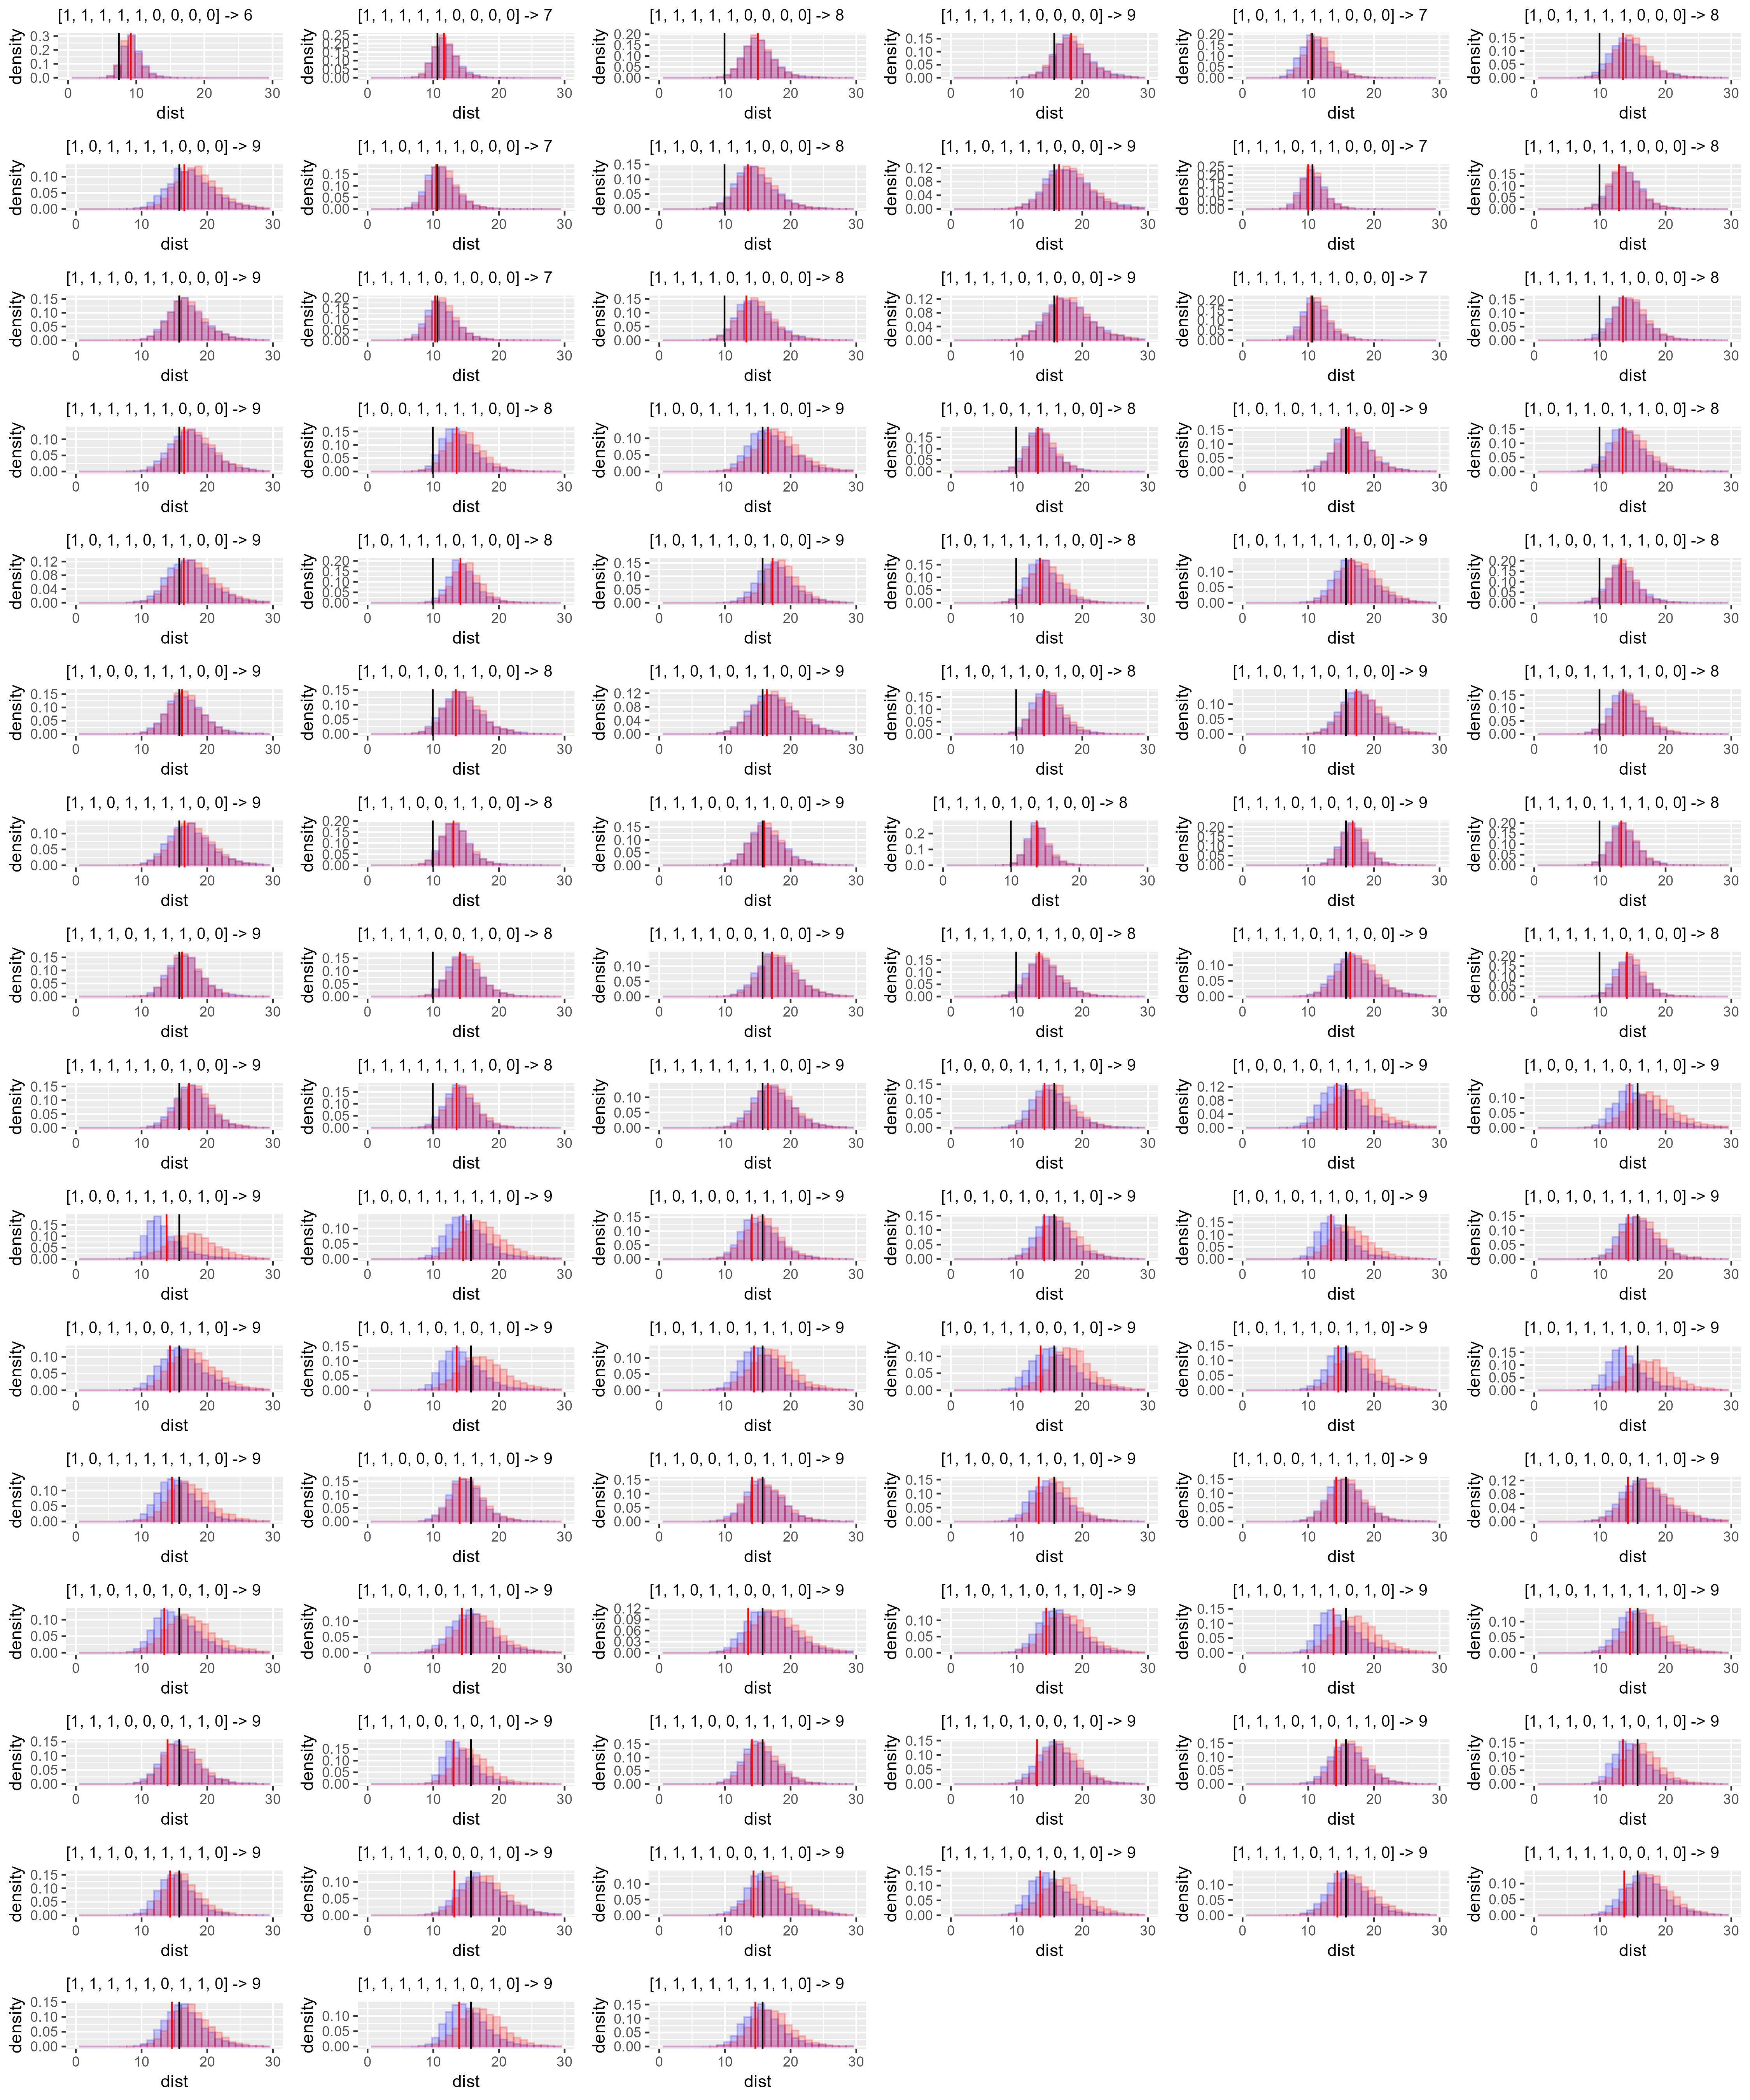
\includegraphics[width=\textwidth]{figures/ch-6/test.png}
  \caption{Comparisons of the forecasted maximum wear according to the two Bayesian models (the blue histogram shows the posterior predictive distribution from the gamma process and the red from the linear general path) and the method of \citet{webb_2020} (red line) with the observed maximum wear (black line). In each plot, the different methods are fit to a subset of the data and forecast a withheld future observation. For example, the plot title `$[1, 0, 1, 1, 1, 1, 1, 0, 0] \rightarrow 8$' indicates that the model was fit to the observations at $(t_1, t_3, t_4, t_5, t_6, t_7)$---leaving out $t_2$, $t_8$, and $t_9$---and that the forecast is generated for $t_8$.}
  \label{fig:beltwear-resampling}
\end{figure}

The comparisons of Figure~\ref{fig:beltwear-resampling} show that the point estimates of \citet{webb_2020} and the maximum a posteriori (MAP) estimates of the Bayesian models are similar, and both reasonably predict the maximum wear measurement. However, the Bayesian MAP estimates are more robust when fewer observations are used to produce the forecasts. Interestingly, the point estimate of \citet{webb_2020} is typically closer to the MAP of the gamma process model than the linear general path model. Comparing the two predictive densities, the gamma process degradation model is much more optimistic than the linear general path. It also looks like it is generally as good or better than the linear general path model at predicting the maximum wear. In general, the observed maximum wear measurement is always contained in both the predictive distributions; with the exception being observation $8$. A closer look at the eighth observation shows that it sits below the seventh observation in many places along the profile, even though it is far from the seventh observation in tonnage. Hence, the eighth observation may well be an extreme outlier. As a reliability practitioner, if you were bing conservative, you would use the predictions of the linear general path model. However, if reducing maintenance cost was important, then effort should be spent to properly validate the two methods since if the gamma process model is in fact a better representation of the true data generating mechanism then making decisions based on the linear general path model's predictions would result in the belt being replaced while it still has remaining useful life and, hence, overspending on maintenance.

\section{Failure time distributions} \label{sec:belt-wear-ft}

The original motivation for forecasting belt wear was to inform practitioners decisions about when to replace the belt. To facilitate this decision, I use the fitted models to generate failure time distributions for the belt conditioned on its current state of degradation. I demonstrate calculating the failure time distributions from the seventh and eighth observation since at the time of the ninth observation there is a non-negligible probability that some point along the belt has already exceeded the soft failure threshold of $25mm$---this is reflected in the max wear predictions for the ninth observation time in Figure~\ref{fig:beltwear-resampling}---and so the failure time distribution is not very helpful. The failure time distribution describes our uncertainty about when the belt will reach the soft failure threshold (the first passage time). Note that unlike the failure time distributions in Chapter~\ref{chap:chapter5}, in this case, the noise in the degradation model for the spline coefficients is important. For some situations, the failure time distribution $F(t)$ has an analytical solution, however, there may be no analytical solution for more complicated processes, and so the failure time distribution must be simulated using Monte Carlo evaluation \citep[p.~504-506]{Meeker2022}. In the case at hand, multiple processes are driving the degradation of each spline coefficient and we must average over the spatial variability along the length of the belt; hence, there is no straightforward analytical solution, and I must simulate the failure time distribution.

\begin{algorithm}
	\caption{Numerical procedure for calculating the failure time distribution conditional on the fitted gamma process model and current state of degradation.}
  \label{algo:ftd}
	\begin{algorithmic}[1]
		\For {each posterior draw}
      \For {$j = 1$ to $1000$}
        \State Starting from most recent filtered spline coefficients.
        \State $\Delta t \gets 0.001$, $t \gets t_I$, $\underline{y}^* \gets \{y^*_{n, I}\}^M_{m = 1}$
        \State Average over the variability along the length of belt.
        \State $\underline{y} \sim \mbox{t}_{10}\left(\underline{y}^*, \underline{y}^* \phi\right)$
        \State Calculate the value of B-spline by multiplying the design matrix by column vector of coefficients.
        \State $\underline{z} \gets B \cdot \underline{y}$
        \While {$Max\left(\underline{z}\right) < 25$}
          \State $\Delta y^*_m \sim Ga\left(\frac{\Delta t}{\nu_m^2}, \frac{1}{\nu_m^2 \mu_m}\right)$
          \State $t \gets t + \Delta t$, $\underline{y}^* \gets \underline{y}^* + \{\Delta y^*_m\}^M_{m = 1}$
          \State $\underline{y} \sim \mbox{t}_{10}\left(\underline{y}^*, \underline{y}^* \phi\right)$
          \State $\underline{z} \gets B \cdot \underline{y}$
        \EndWhile
        \State $FT[j] \gets t$
      \EndFor
      \State Calculate the empirical cdf from $FT$.
    \EndFor
	\end{algorithmic} 
\end{algorithm} 

To calculate the failure time numerically from the gamma process model I use the procedure in \textit{Algorithm}~\ref{algo:ftd}. For each of the $12000$ posterior draws, I simulate $1000$ pathways from the most recent observation until soft failure. Each pathway is simulated by incrementing the GP forward by time steps of $0.001$ and averaging over the variability along the length of the belt until the degradation at some point exceeds the soft failure threshold. Using the times at which each of $1000$ simulated pathways cross the soft failure threshold, I construct an empirical failure time CDF. The result of \textit{Algorithm}~\ref{algo:ftd} is $12000$ empirical CDFs---one for each of the posterior draws. I construct the failure time distribution from the general path model in the same way, except that when I calculate the filtered values of the spline coefficients, I do so using the deterministic degradation function $\underline{y}^* = \underline{\mu} t$. The distributions of the CDFs are shown in Figure~\ref{fig:beltwear-ft-gp} for the gamma process and Figure~\ref{fig:beltwear-ft-lm} for the general path model fitted to the first seven observations (Fig.~(a) and~\ref{fig:beltwear-ft-lm}~(a) respectively) and for the first eight observations (Fig.~\ref{fig:beltwear-ft-gp}~(b) and~\ref{fig:beltwear-ft-lm}~(b) respectively). The average CDF is shown as a black line and the $0.5, 0.8$, and $0.95$ uncertainty intervals in different shades of blue. From the distributions of the failure time CDFs, we can quickly interpret the risk of the soft failure of the belt as we delay the replacement time.

\begin{figure}
  \centering
  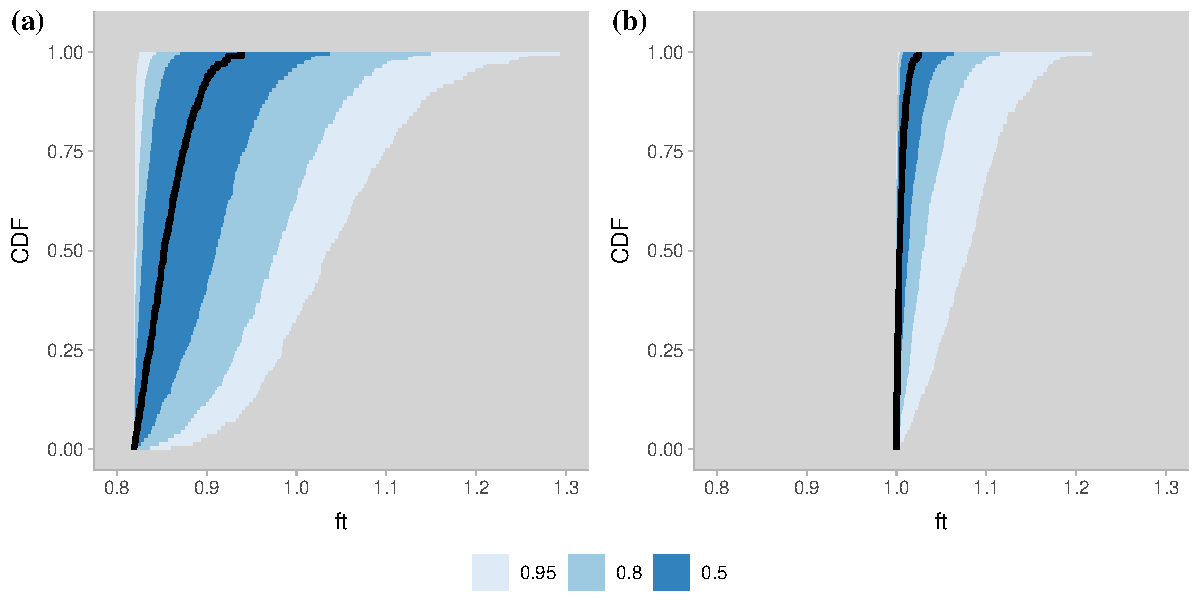
\includegraphics[width=\textwidth]{figures/ch-6/belt_wear_failuretime_CDF_gp.pdf}
  \caption{The failure time CDFs generated from the posterior of the gamma process model conditioned on the first (a) seven and (b) eight observations. The median CDF is indicated by the black line and the uncertainty intervals are shown by the deferent shades of blue ribbons.}
  \label{fig:beltwear-ft-gp}
\end{figure}

Remembering that maintenance decisions are made in the context of the whole business, not just the specific asses; a reliability engineer may plan to replace belts when there is a 25\% chance that they have exceeded the soft failure threshold---remembering that soft failure means that the belt is still technically operational. At the time of the seventh observation, for this particular belt that I have analysed, the predicted time from the gamma process (linear general path) model that there is a 25\% chance of soft failure is at $0.82$($0.81$) tonnes with a lower and upper bound of $0.75$ and $0.95$($0.74$ and $0.90$) respectively. Say there are two planned maintenance shutdowns for the particular conveyor coming up; a reliability practitioner can use this distribution to inform which shutdown they should replace the belt in. The uncertainty intervals can also help to select one belt over another. Furthermore, since the failure time prediction is with respect to tonnes, the reliability practitioner could look at reducing (or even increasing) the planned operation of the belt to manage the probability of soft failure at the calendar time of the maintenance shutdown. Once we observed the eighth set of measurements, our belief is then updated, and the estimate for the time at which there is a 25\% chance of soft failure becomes $0.95$ ($0.85$) tonnes, and the lower and upper uncertainty bounds become $0.83$ and $1.09$ ($0.83$ and $0.91$), respectively. Using this updated belief, the reliability practitioner could re-evaluate their decision and make last-minute changes to a shutdown plan while formally managing risk.

\begin{figure}
  \centering
  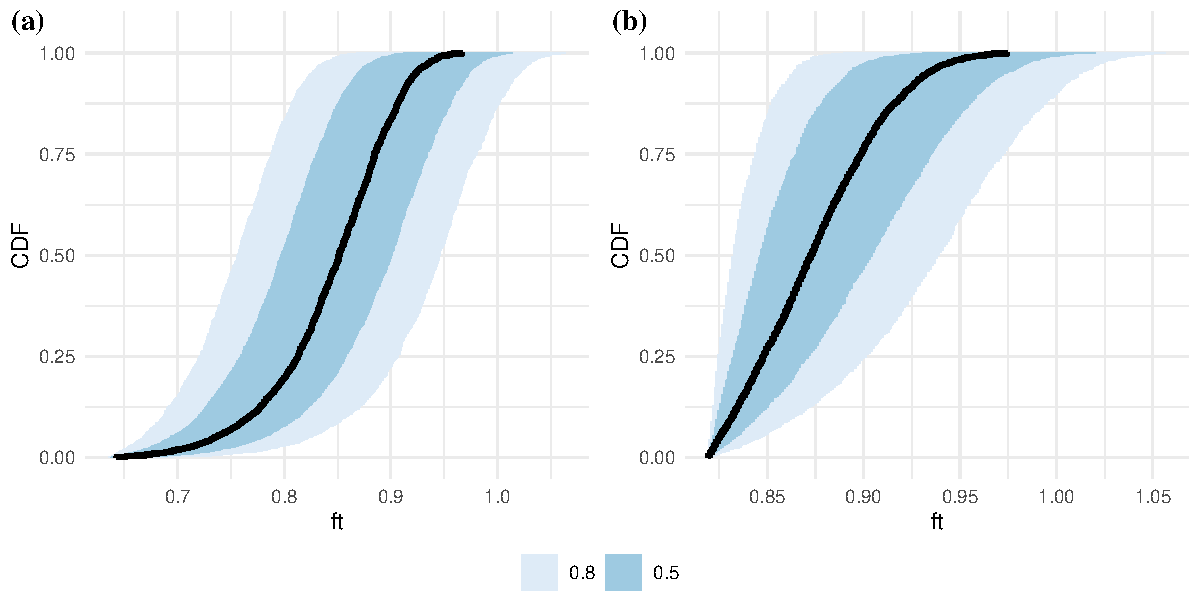
\includegraphics[width=\textwidth]{figures/ch-6/belt_wear_failuretime_CDF_lm.pdf}
  \caption{The failure time CDFs generated from the posterior of the linear general path model conditioned on the first (a) seven and (b) eight observations. The median CDF is indicated by the black line and the uncertainty intervals are shown by the deferent shades of blue ribbons.}
  \label{fig:beltwear-ft-lm}
\end{figure}

\section{Discussions} \label{sec:belt-wear-discussion}

In this chapter, I've constructed, fit, evaluated, and compared two BHMs for conveyor belt wear, and, in doing so, demonstrated an end-to-end example of the Bayesian workflow for an applied problem in the mining industry. In the data models for the two BHMs, I extend FDA to degradation modelling in order to model a degrading surface. In the two process models, I compared the noisy gamma process model from chapters~\ref{chap:chapter4} and~\ref{chap:chapter5} with a linear general path model. Lastly, in the parameter models, I show how historical belt wear data can be used to inform the analysis of the current belt through an informative prior. I compare the two models with one another through the expected log score of N step ahead predictions and also compare them alongside the method of \cite{webb_2020} in their ability to predict the maximum wear measurement. Lastly, I've shown how to construct failure time distributions based on the current degradation of the belt for the two BHMs. In this last section, I distil the main points of the chapter, discuss the advantages and limitations of the BHM models I have explored and point to areas of future work.

The comparison of the two Bayesian models shows that while both models appear to have reasonably fit the data, the linear general path model is a better predictive model for the overall belt's wear. However, when the two models are compared based on their ability to predict the maximum wear observation, which defines the soft failure of the belt, both models' predictions appear reasonable when compared with the observed data and the gamma process model's forecasts are far more optimistic. Consequently, this is also reflected in the failure time distributions generated from the two models. If these models were to be implemented in practice, it would be worth investing in collecting more detailed data for a short period of time to properly validate the models---i.e. collecting wear profiles more frequently and measuring more than one location along the belt's length at each time.

An added advantage of the BHM structure applied to belt wear is that the structure can easily incorporate additional observations into the model without the model becoming over-parameterised and can take full advantage of such extra information to reduce the uncertainty of parameter estimates and predictions. This is particularly true for the noisy gamma process model. For example, if we were to have a much finer grid of measurements across the width of the belt's surface at each observation time, these measurements would still be summarised by the same number of spline coefficients. So, the result would be better uncertainty quantification of $\sigma$ with no additional parameters in the lower levels of the hierarchical model. Alternatively, if more than one functional observation was recorded at each observation time, this could be incorporated by drawing more than one realisation of the noisy spline coefficients. To elaborate, instead of a single set of noisy spline coefficients at each time, we could use $y_{j, i, m} \sim N(y^*_{i, m}, y^*_{i, m}\phi)$, where the new subscript $j$ identifies the different functional observation at time $t_i$. The result would be better identification of $\phi$---the spatial variation in wear profiles along the length of the belt---and subsequently a more precise filtered estimate of the $y^*_{i, m}$. Lastly, if observations were collected more frequently, then the finer temporal resolution would better identify the `jumpiness' of the gamma process---i.e. $\nu$ would be estimated more precisely---which refines the uncertainty quantification of the forecasts from the gamma process. 

An alternative extension of the data would be if the set of UT measurements at each time were two-dimensional. Here, we have shown an application of this model to a one-dimensional surface; however, the method could easily be extended to a two-dimensional wearing surface by using two-dimensional spatial basis functions such as in \citet[p. 84]{wikle_2019}. For the case of belt wear, we could extend the model in this way if there were multiple functional observations at each time, and we knew the location along the length of the belt of each observation. By expanding the model to two dimensions, the method could be applied to the degradation of many other assets---for example, the wear liners in transfer station shoots or haul truck beds.

As I touched on briefly when discussing the prior predictive checks in Section~\ref{sec:belt_wear_priors}, I have made the simplifying assumption that the spline coefficients are independent of one another. In doing so, we neglect any large-scale spatial structure in the wear profiles. For both prior and posterior predictive checks, if we simulate a single belt profile, it will look unrealistically `wiggly'. Although the B-spline accounts for small-scale spatial structure in the UT measurements, the assumed independence of the spline coefficients means that there is no way to capture any large-scale spacial structure. In reality, we would expect neighbouring coefficients to behave somewhat similarly. A possible way of accounting for this large-scale spatial correlation would be to include a spatial random effect, which would most likely result in better uncertainty quantification in the parameter estimates and forecasts since we are adding information about the underlying process through the model's structure. One hurdle to implementing a spatial random effect in the gamma process model is there is no straightforward way of coercing correlation in the jumps of multiple gamma processes. This would be an interesting area for future work. Because of this hurdle, it may be simpler to implement large-scale spatial structure in the linear model. This could be done using a conditional autoregressive structure. Nevertheless, the simplifying assumption of independence appears acceptable since the `wiggliness' of the individual realisations is `washed out' when I average over all of the posterior draws, making any predictions look smooth, such as in Fig.~\ref{fig:beltwear-forecasts}.

When confronted with analysing complicated, small, and messy datasets---something very common in reliability and condition monitoring---a very natural approach is to simplify the data and apply methods we are familiar with, such as regression. However, here we have demonstrated that if we instead take the time to think deeply about how the data arise and what extra knowledge we possess about the data-generating process, we can construct statistical models that take full advantage of all the information available in both the data and our understanding of the problem. In doing so, we get more detailed predictions and defensible uncertainty qualification for the reliability predictions and accompanying maintenance decisions.